\documentclass[twoside]{book}

% Packages required by doxygen
\usepackage{fixltx2e}
\usepackage{calc}
\usepackage{doxygen}
\usepackage[export]{adjustbox} % also loads graphicx
\usepackage{graphicx}
\usepackage[utf8]{inputenc}
\usepackage{makeidx}
\usepackage{multicol}
\usepackage{multirow}
\PassOptionsToPackage{warn}{textcomp}
\usepackage{textcomp}
\usepackage[nointegrals]{wasysym}
\usepackage[table]{xcolor}

% NLS support packages
\usepackage[ngerman]{babel}

% Font selection
\usepackage[T1]{fontenc}
\usepackage[scaled=.90]{helvet}
\usepackage{courier}
\usepackage{amssymb}
\usepackage{sectsty}
\renewcommand{\familydefault}{\sfdefault}
\allsectionsfont{%
  \fontseries{bc}\selectfont%
  \color{darkgray}%
}
\renewcommand{\DoxyLabelFont}{%
  \fontseries{bc}\selectfont%
  \color{darkgray}%
}
\newcommand{\+}{\discretionary{\mbox{\scriptsize$\hookleftarrow$}}{}{}}

% Page & text layout
\usepackage{geometry}
\geometry{%
  a4paper,%
  top=2.5cm,%
  bottom=2.5cm,%
  left=2.5cm,%
  right=2.5cm%
}
\tolerance=750
\hfuzz=15pt
\hbadness=750
\setlength{\emergencystretch}{15pt}
\setlength{\parindent}{0cm}
\setlength{\parskip}{3ex plus 2ex minus 2ex}
\makeatletter
\renewcommand{\paragraph}{%
  \@startsection{paragraph}{4}{0ex}{-1.0ex}{1.0ex}{%
    \normalfont\normalsize\bfseries\SS@parafont%
  }%
}
\renewcommand{\subparagraph}{%
  \@startsection{subparagraph}{5}{0ex}{-1.0ex}{1.0ex}{%
    \normalfont\normalsize\bfseries\SS@subparafont%
  }%
}
\makeatother

% Headers & footers
\usepackage{fancyhdr}
\pagestyle{fancyplain}
\fancyhead[LE]{\fancyplain{}{\bfseries\thepage}}
\fancyhead[CE]{\fancyplain{}{}}
\fancyhead[RE]{\fancyplain{}{\bfseries\leftmark}}
\fancyhead[LO]{\fancyplain{}{\bfseries\rightmark}}
\fancyhead[CO]{\fancyplain{}{}}
\fancyhead[RO]{\fancyplain{}{\bfseries\thepage}}
\fancyfoot[LE]{\fancyplain{}{}}
\fancyfoot[CE]{\fancyplain{}{}}
\fancyfoot[RE]{\fancyplain{}{\bfseries\scriptsize Erzeugt von Doxygen }}
\fancyfoot[LO]{\fancyplain{}{\bfseries\scriptsize Erzeugt von Doxygen }}
\fancyfoot[CO]{\fancyplain{}{}}
\fancyfoot[RO]{\fancyplain{}{}}
\renewcommand{\footrulewidth}{0.4pt}
\renewcommand{\chaptermark}[1]{%
  \markboth{#1}{}%
}
\renewcommand{\sectionmark}[1]{%
  \markright{\thesection\ #1}%
}

% Indices & bibliography
\usepackage{natbib}
\usepackage[titles]{tocloft}
\setcounter{tocdepth}{3}
\setcounter{secnumdepth}{5}
\makeindex

% Hyperlinks (required, but should be loaded last)
\usepackage{ifpdf}
\ifpdf
  \usepackage[pdftex,pagebackref=true]{hyperref}
\else
  \usepackage[ps2pdf,pagebackref=true]{hyperref}
\fi
\hypersetup{%
  colorlinks=true,%
  linkcolor=blue,%
  citecolor=blue,%
  unicode%
}

% Custom commands
\newcommand{\clearemptydoublepage}{%
  \newpage{\pagestyle{empty}\cleardoublepage}%
}

\usepackage{caption}
\captionsetup{labelsep=space,justification=centering,font={bf},singlelinecheck=off,skip=4pt,position=top}

%===== C O N T E N T S =====

\begin{document}

% Titlepage & ToC
\hypersetup{pageanchor=false,
             bookmarksnumbered=true,
             pdfencoding=unicode
            }
\pagenumbering{alph}
\begin{titlepage}
\vspace*{7cm}
\begin{center}%
{\Large My Project }\\
\vspace*{1cm}
{\large Erzeugt von Doxygen 1.8.14}\\
\end{center}
\end{titlepage}
\clearemptydoublepage
\pagenumbering{roman}
\tableofcontents
\clearemptydoublepage
\pagenumbering{arabic}
\hypersetup{pageanchor=true}

%--- Begin generated contents ---
\chapter{Verzeichnis der Namensbereiche}
\section{Liste aller Namensbereiche}
Liste aller Namensbereiche mit Kurzbeschreibung\+:\begin{DoxyCompactList}
\item\contentsline{section}{\mbox{\hyperlink{namespacecepstrum}{cepstrum}} }{\pageref{namespacecepstrum}}{}
\item\contentsline{section}{\mbox{\hyperlink{namespace_perceptron}{Perceptron}} }{\pageref{namespace_perceptron}}{}
\item\contentsline{section}{\mbox{\hyperlink{namespace_pretty_table}{Pretty\+Table}} }{\pageref{namespace_pretty_table}}{}
\item\contentsline{section}{\mbox{\hyperlink{namespaceprint}{print}} }{\pageref{namespaceprint}}{}
\item\contentsline{section}{\mbox{\hyperlink{namespacesda__help}{sda\+\_\+help}} }{\pageref{namespacesda__help}}{}
\item\contentsline{section}{\mbox{\hyperlink{namespaceshowres}{showres}} }{\pageref{namespaceshowres}}{}
\item\contentsline{section}{\mbox{\hyperlink{namespacesounddata}{sounddata}} }{\pageref{namespacesounddata}}{}
\item\contentsline{section}{\mbox{\hyperlink{namespacetsv__helper}{tsv\+\_\+helper}} }{\pageref{namespacetsv__helper}}{}
\end{DoxyCompactList}

\chapter{Hierarchie-\/\+Verzeichnis}
\section{Klassenhierarchie}
Die Liste der Ableitungen ist -\/mit Einschränkungen-\/ alphabetisch sortiert\+:\begin{DoxyCompactList}
\item list\begin{DoxyCompactList}
\item \contentsline{section}{Pretty\+Table.\+Pretty\+Table}{\pageref{class_pretty_table_1_1_pretty_table}}{}
\end{DoxyCompactList}
\item object\begin{DoxyCompactList}
\item \contentsline{section}{Perceptron.\+Perceptron}{\pageref{class_perceptron_1_1_perceptron}}{}
\end{DoxyCompactList}
\item \contentsline{section}{sounddata.\+Sounddata}{\pageref{classsounddata_1_1_sounddata}}{}
\end{DoxyCompactList}

\chapter{Klassen-\/\+Verzeichnis}
\section{Auflistung der Klassen}
Hier folgt die Aufzählung aller Klassen, Strukturen, Varianten und Schnittstellen mit einer Kurzbeschreibung\+:\begin{DoxyCompactList}
\item\contentsline{section}{\mbox{\hyperlink{class_perceptron_1_1_perceptron}{Perceptron.\+Perceptron}} }{\pageref{class_perceptron_1_1_perceptron}}{}
\item\contentsline{section}{\mbox{\hyperlink{class_pretty_table_1_1_pretty_table}{Pretty\+Table.\+Pretty\+Table}} }{\pageref{class_pretty_table_1_1_pretty_table}}{}
\item\contentsline{section}{\mbox{\hyperlink{classsounddata_1_1_sounddata}{sounddata.\+Sounddata}} \\*Dokumentation für die Klasse \mbox{\hyperlink{classsounddata_1_1_sounddata}{Sounddata}} }{\pageref{classsounddata_1_1_sounddata}}{}
\end{DoxyCompactList}

\chapter{Datei-\/\+Verzeichnis}
\section{Auflistung der Dateien}
Hier folgt die Aufzählung aller Dateien mit einer Kurzbeschreibung\+:\begin{DoxyCompactList}
\item\contentsline{section}{C\+:/\+Users/flach/\+Documents/\+Lehre/\+Module/\+T\+S\+V/notebooks/\+L\+V\+\_\+\+T\+S\+V\+\_\+repos/aktuell/functions/\mbox{\hyperlink{cepstrum_8py}{cepstrum.\+py}} }{\pageref{cepstrum_8py}}{}
\item\contentsline{section}{C\+:/\+Users/flach/\+Documents/\+Lehre/\+Module/\+T\+S\+V/notebooks/\+L\+V\+\_\+\+T\+S\+V\+\_\+repos/aktuell/functions/\mbox{\hyperlink{_perceptron_8py}{Perceptron.\+py}} }{\pageref{_perceptron_8py}}{}
\item\contentsline{section}{C\+:/\+Users/flach/\+Documents/\+Lehre/\+Module/\+T\+S\+V/notebooks/\+L\+V\+\_\+\+T\+S\+V\+\_\+repos/aktuell/functions/\mbox{\hyperlink{_pretty_table_8py}{Pretty\+Table.\+py}} }{\pageref{_pretty_table_8py}}{}
\item\contentsline{section}{C\+:/\+Users/flach/\+Documents/\+Lehre/\+Module/\+T\+S\+V/notebooks/\+L\+V\+\_\+\+T\+S\+V\+\_\+repos/aktuell/functions/\mbox{\hyperlink{print_8py}{print.\+py}} }{\pageref{print_8py}}{}
\item\contentsline{section}{C\+:/\+Users/flach/\+Documents/\+Lehre/\+Module/\+T\+S\+V/notebooks/\+L\+V\+\_\+\+T\+S\+V\+\_\+repos/aktuell/functions/\mbox{\hyperlink{sda__help_8py}{sda\+\_\+help.\+py}} }{\pageref{sda__help_8py}}{}
\item\contentsline{section}{C\+:/\+Users/flach/\+Documents/\+Lehre/\+Module/\+T\+S\+V/notebooks/\+L\+V\+\_\+\+T\+S\+V\+\_\+repos/aktuell/functions/\mbox{\hyperlink{showres_8py}{showres.\+py}} }{\pageref{showres_8py}}{}
\item\contentsline{section}{C\+:/\+Users/flach/\+Documents/\+Lehre/\+Module/\+T\+S\+V/notebooks/\+L\+V\+\_\+\+T\+S\+V\+\_\+repos/aktuell/functions/\mbox{\hyperlink{sounddata_8py}{sounddata.\+py}} }{\pageref{sounddata_8py}}{}
\item\contentsline{section}{C\+:/\+Users/flach/\+Documents/\+Lehre/\+Module/\+T\+S\+V/notebooks/\+L\+V\+\_\+\+T\+S\+V\+\_\+repos/aktuell/functions/\mbox{\hyperlink{tsv__helper_8py}{tsv\+\_\+helper.\+py}} }{\pageref{tsv__helper_8py}}{}
\end{DoxyCompactList}

\chapter{Dokumentation der Namensbereiche}
\hypertarget{namespacecepstrum}{}\section{cepstrum-\/\+Namensbereichsreferenz}
\label{namespacecepstrum}\index{cepstrum@{cepstrum}}
\subsection*{Funktionen}
\begin{DoxyCompactItemize}
\item 
def \mbox{\hyperlink{namespacecepstrum_af44fa6a9e5f5e8db043cb60b38894085}{read\+\_\+show\+\_\+sig}} (file\+\_\+name, sig\+\_\+dur)
\item 
def \mbox{\hyperlink{namespacecepstrum_ae9a55612bcfeaa372d11036a16b98527}{show\+\_\+sig}} (signal, sig\+\_\+dur, file\+\_\+name)
\item 
def \mbox{\hyperlink{namespacecepstrum_ab6397c51bd13894929df2b4c206fecfa}{wind\+\_\+sig}} (frame\+\_\+size, frame\+\_\+stride, sample\+\_\+rate, signal)
\item 
def \mbox{\hyperlink{namespacecepstrum_a3db8285f132510ae674c893a651ca971}{show\+\_\+spectrogram}} (frames, sig\+\_\+dur, sample\+\_\+rate)
\item 
def \mbox{\hyperlink{namespacecepstrum_ae0a1b2c79db9e80e8dfe58fd9dfb9ad6}{mel\+\_\+spec}} (nfilt, sample\+\_\+rate, N\+F\+FT, sig\+\_\+frames)
\item 
def \mbox{\hyperlink{namespacecepstrum_a3e21b1c622287001e82e62c0c64d0643}{show\+\_\+melspec}} (mel\+\_\+frames, sig\+\_\+dur, nfilt)
\item 
def \mbox{\hyperlink{namespacecepstrum_a43917229e1efedf7a3439fdfc6b2890a}{show\+\_\+mfcc}} (mfcc, sig\+\_\+dur, num\+\_\+ceps)
\end{DoxyCompactItemize}


\subsection{Dokumentation der Funktionen}
\mbox{\Hypertarget{namespacecepstrum_ae0a1b2c79db9e80e8dfe58fd9dfb9ad6}\label{namespacecepstrum_ae0a1b2c79db9e80e8dfe58fd9dfb9ad6}} 
\index{cepstrum@{cepstrum}!mel\+\_\+spec@{mel\+\_\+spec}}
\index{mel\+\_\+spec@{mel\+\_\+spec}!cepstrum@{cepstrum}}
\subsubsection{\texorpdfstring{mel\+\_\+spec()}{mel\_spec()}}
{\footnotesize\ttfamily def cepstrum.\+mel\+\_\+spec (\begin{DoxyParamCaption}\item[{}]{nfilt,  }\item[{}]{sample\+\_\+rate,  }\item[{}]{N\+F\+FT,  }\item[{}]{sig\+\_\+frames }\end{DoxyParamCaption})}

\mbox{\Hypertarget{namespacecepstrum_af44fa6a9e5f5e8db043cb60b38894085}\label{namespacecepstrum_af44fa6a9e5f5e8db043cb60b38894085}} 
\index{cepstrum@{cepstrum}!read\+\_\+show\+\_\+sig@{read\+\_\+show\+\_\+sig}}
\index{read\+\_\+show\+\_\+sig@{read\+\_\+show\+\_\+sig}!cepstrum@{cepstrum}}
\subsubsection{\texorpdfstring{read\+\_\+show\+\_\+sig()}{read\_show\_sig()}}
{\footnotesize\ttfamily def cepstrum.\+read\+\_\+show\+\_\+sig (\begin{DoxyParamCaption}\item[{}]{file\+\_\+name,  }\item[{}]{sig\+\_\+dur }\end{DoxyParamCaption})}

\mbox{\Hypertarget{namespacecepstrum_a3e21b1c622287001e82e62c0c64d0643}\label{namespacecepstrum_a3e21b1c622287001e82e62c0c64d0643}} 
\index{cepstrum@{cepstrum}!show\+\_\+melspec@{show\+\_\+melspec}}
\index{show\+\_\+melspec@{show\+\_\+melspec}!cepstrum@{cepstrum}}
\subsubsection{\texorpdfstring{show\+\_\+melspec()}{show\_melspec()}}
{\footnotesize\ttfamily def cepstrum.\+show\+\_\+melspec (\begin{DoxyParamCaption}\item[{}]{mel\+\_\+frames,  }\item[{}]{sig\+\_\+dur,  }\item[{}]{nfilt }\end{DoxyParamCaption})}

\mbox{\Hypertarget{namespacecepstrum_a43917229e1efedf7a3439fdfc6b2890a}\label{namespacecepstrum_a43917229e1efedf7a3439fdfc6b2890a}} 
\index{cepstrum@{cepstrum}!show\+\_\+mfcc@{show\+\_\+mfcc}}
\index{show\+\_\+mfcc@{show\+\_\+mfcc}!cepstrum@{cepstrum}}
\subsubsection{\texorpdfstring{show\+\_\+mfcc()}{show\_mfcc()}}
{\footnotesize\ttfamily def cepstrum.\+show\+\_\+mfcc (\begin{DoxyParamCaption}\item[{}]{mfcc,  }\item[{}]{sig\+\_\+dur,  }\item[{}]{num\+\_\+ceps }\end{DoxyParamCaption})}

\mbox{\Hypertarget{namespacecepstrum_ae9a55612bcfeaa372d11036a16b98527}\label{namespacecepstrum_ae9a55612bcfeaa372d11036a16b98527}} 
\index{cepstrum@{cepstrum}!show\+\_\+sig@{show\+\_\+sig}}
\index{show\+\_\+sig@{show\+\_\+sig}!cepstrum@{cepstrum}}
\subsubsection{\texorpdfstring{show\+\_\+sig()}{show\_sig()}}
{\footnotesize\ttfamily def cepstrum.\+show\+\_\+sig (\begin{DoxyParamCaption}\item[{}]{signal,  }\item[{}]{sig\+\_\+dur,  }\item[{}]{file\+\_\+name }\end{DoxyParamCaption})}

\mbox{\Hypertarget{namespacecepstrum_a3db8285f132510ae674c893a651ca971}\label{namespacecepstrum_a3db8285f132510ae674c893a651ca971}} 
\index{cepstrum@{cepstrum}!show\+\_\+spectrogram@{show\+\_\+spectrogram}}
\index{show\+\_\+spectrogram@{show\+\_\+spectrogram}!cepstrum@{cepstrum}}
\subsubsection{\texorpdfstring{show\+\_\+spectrogram()}{show\_spectrogram()}}
{\footnotesize\ttfamily def cepstrum.\+show\+\_\+spectrogram (\begin{DoxyParamCaption}\item[{}]{frames,  }\item[{}]{sig\+\_\+dur,  }\item[{}]{sample\+\_\+rate }\end{DoxyParamCaption})}

\mbox{\Hypertarget{namespacecepstrum_ab6397c51bd13894929df2b4c206fecfa}\label{namespacecepstrum_ab6397c51bd13894929df2b4c206fecfa}} 
\index{cepstrum@{cepstrum}!wind\+\_\+sig@{wind\+\_\+sig}}
\index{wind\+\_\+sig@{wind\+\_\+sig}!cepstrum@{cepstrum}}
\subsubsection{\texorpdfstring{wind\+\_\+sig()}{wind\_sig()}}
{\footnotesize\ttfamily def cepstrum.\+wind\+\_\+sig (\begin{DoxyParamCaption}\item[{}]{frame\+\_\+size,  }\item[{}]{frame\+\_\+stride,  }\item[{}]{sample\+\_\+rate,  }\item[{}]{signal }\end{DoxyParamCaption})}


\hypertarget{namespace_perceptron}{}\section{Perceptron-\/\+Namensbereichsreferenz}
\label{namespace_perceptron}\index{Perceptron@{Perceptron}}
\subsection*{Klassen}
\begin{DoxyCompactItemize}
\item 
class \mbox{\hyperlink{class_perceptron_1_1_perceptron}{Perceptron}}
\end{DoxyCompactItemize}

\hypertarget{namespace_pretty_table}{}\section{Pretty\+Table-\/\+Namensbereichsreferenz}
\label{namespace_pretty_table}\index{Pretty\+Table@{Pretty\+Table}}
\subsection*{Klassen}
\begin{DoxyCompactItemize}
\item 
class \mbox{\hyperlink{class_pretty_table_1_1_pretty_table}{Pretty\+Table}}
\end{DoxyCompactItemize}

\hypertarget{namespaceprint}{}\section{print-\/\+Namensbereichsreferenz}
\label{namespaceprint}\index{print@{print}}
\subsection*{Variablen}
\begin{DoxyCompactItemize}
\item 
\mbox{\hyperlink{namespaceprint_a8080002122fd53cadd2b548837d037aa}{fig}} = plt.\+figure(figsize=(10,10))
\item 
\mbox{\hyperlink{namespaceprint_a980229015cfaa5dda779f5e1df7e4013}{ax}} = fig.\+add\+\_\+subplot(1, 1, 1, projection=\textquotesingle{}3d\textquotesingle{})
\item 
\mbox{\hyperlink{namespaceprint_affd04964e07d6931f5b7f92164b9b99f}{X}} = np.\+arange(-\/10, 10, 0.\+25)
\item 
\mbox{\hyperlink{namespaceprint_aab512732eb82cbe258baa68f9f9add63}{Y}} = np.\+arange(-\/10, 10, 0.\+25)
\item 
int \mbox{\hyperlink{namespaceprint_a0d1f4b3564b3a18949e4a9d42c0fe83b}{mu}} = -\/2
\item 
float \mbox{\hyperlink{namespaceprint_a1efc77cd3bf0d758b07ec8e2b2c71c6b}{sig}} = 1.\+5
\item 
int \mbox{\hyperlink{namespaceprint_acc02b068ba7893cb51896817458953b1}{Z1}} = 1/(\mbox{\hyperlink{namespaceprint_a1efc77cd3bf0d758b07ec8e2b2c71c6b}{sig}}$\ast$np.\+sqrt(2$\ast$np.\+pi))$\ast$np.\+exp(-\/(\mbox{\hyperlink{namespaceprint_affd04964e07d6931f5b7f92164b9b99f}{X}} -\/ \mbox{\hyperlink{namespaceprint_a0d1f4b3564b3a18949e4a9d42c0fe83b}{mu}})$\ast$$\ast$2/(2$\ast$\mbox{\hyperlink{namespaceprint_a1efc77cd3bf0d758b07ec8e2b2c71c6b}{sig}}$\ast$$\ast$2))$\ast$\textbackslash{}
\item 
int \mbox{\hyperlink{namespaceprint_a09064592a1be5db47dee477a81ae8bf3}{Z2}} = 1/(\mbox{\hyperlink{namespaceprint_a1efc77cd3bf0d758b07ec8e2b2c71c6b}{sig}}$\ast$np.\+sqrt(2$\ast$np.\+pi))$\ast$np.\+exp(-\/(\mbox{\hyperlink{namespaceprint_affd04964e07d6931f5b7f92164b9b99f}{X}} -\/ \mbox{\hyperlink{namespaceprint_a0d1f4b3564b3a18949e4a9d42c0fe83b}{mu}})$\ast$$\ast$2/(2$\ast$\mbox{\hyperlink{namespaceprint_a1efc77cd3bf0d758b07ec8e2b2c71c6b}{sig}}$\ast$$\ast$2))$\ast$\textbackslash{}
\item 
int \mbox{\hyperlink{namespaceprint_a9433aedd977f6182d23edaf955e46742}{Z}} = 4$\ast$\mbox{\hyperlink{namespaceprint_acc02b068ba7893cb51896817458953b1}{Z1}} + 5$\ast$\mbox{\hyperlink{namespaceprint_a09064592a1be5db47dee477a81ae8bf3}{Z2}}
\item 
\mbox{\hyperlink{namespaceprint_a25485f663d582df21114be2f03bad0e0}{zdir}}
\item 
\mbox{\hyperlink{namespaceprint_a63b63e4e6ea6a9b03c0e161424d919e8}{offset}}
\item 
\mbox{\hyperlink{namespaceprint_a811f3257310281e4a58230ebd65dcc71}{levels}}
\item 
\mbox{\hyperlink{namespaceprint_a4c39ba09ea1a62ecd2fc116b9ef27c42}{cmap}}
\end{DoxyCompactItemize}


\subsection{Variablen-\/\+Dokumentation}
\mbox{\Hypertarget{namespaceprint_a980229015cfaa5dda779f5e1df7e4013}\label{namespaceprint_a980229015cfaa5dda779f5e1df7e4013}} 
\index{print@{print}!ax@{ax}}
\index{ax@{ax}!print@{print}}
\subsubsection{\texorpdfstring{ax}{ax}}
{\footnotesize\ttfamily print.\+ax = fig.\+add\+\_\+subplot(1, 1, 1, projection=\textquotesingle{}3d\textquotesingle{})}

\mbox{\Hypertarget{namespaceprint_a4c39ba09ea1a62ecd2fc116b9ef27c42}\label{namespaceprint_a4c39ba09ea1a62ecd2fc116b9ef27c42}} 
\index{print@{print}!cmap@{cmap}}
\index{cmap@{cmap}!print@{print}}
\subsubsection{\texorpdfstring{cmap}{cmap}}
{\footnotesize\ttfamily print.\+cmap}

\mbox{\Hypertarget{namespaceprint_a8080002122fd53cadd2b548837d037aa}\label{namespaceprint_a8080002122fd53cadd2b548837d037aa}} 
\index{print@{print}!fig@{fig}}
\index{fig@{fig}!print@{print}}
\subsubsection{\texorpdfstring{fig}{fig}}
{\footnotesize\ttfamily print.\+fig = plt.\+figure(figsize=(10,10))}

\mbox{\Hypertarget{namespaceprint_a811f3257310281e4a58230ebd65dcc71}\label{namespaceprint_a811f3257310281e4a58230ebd65dcc71}} 
\index{print@{print}!levels@{levels}}
\index{levels@{levels}!print@{print}}
\subsubsection{\texorpdfstring{levels}{levels}}
{\footnotesize\ttfamily print.\+levels}

\mbox{\Hypertarget{namespaceprint_a0d1f4b3564b3a18949e4a9d42c0fe83b}\label{namespaceprint_a0d1f4b3564b3a18949e4a9d42c0fe83b}} 
\index{print@{print}!mu@{mu}}
\index{mu@{mu}!print@{print}}
\subsubsection{\texorpdfstring{mu}{mu}}
{\footnotesize\ttfamily int print.\+mu = -\/2}

\mbox{\Hypertarget{namespaceprint_a63b63e4e6ea6a9b03c0e161424d919e8}\label{namespaceprint_a63b63e4e6ea6a9b03c0e161424d919e8}} 
\index{print@{print}!offset@{offset}}
\index{offset@{offset}!print@{print}}
\subsubsection{\texorpdfstring{offset}{offset}}
{\footnotesize\ttfamily print.\+offset}

\mbox{\Hypertarget{namespaceprint_a1efc77cd3bf0d758b07ec8e2b2c71c6b}\label{namespaceprint_a1efc77cd3bf0d758b07ec8e2b2c71c6b}} 
\index{print@{print}!sig@{sig}}
\index{sig@{sig}!print@{print}}
\subsubsection{\texorpdfstring{sig}{sig}}
{\footnotesize\ttfamily int print.\+sig = 1.\+5}

\mbox{\Hypertarget{namespaceprint_affd04964e07d6931f5b7f92164b9b99f}\label{namespaceprint_affd04964e07d6931f5b7f92164b9b99f}} 
\index{print@{print}!X@{X}}
\index{X@{X}!print@{print}}
\subsubsection{\texorpdfstring{X}{X}}
{\footnotesize\ttfamily print.\+X = np.\+arange(-\/10, 10, 0.\+25)}

\mbox{\Hypertarget{namespaceprint_aab512732eb82cbe258baa68f9f9add63}\label{namespaceprint_aab512732eb82cbe258baa68f9f9add63}} 
\index{print@{print}!Y@{Y}}
\index{Y@{Y}!print@{print}}
\subsubsection{\texorpdfstring{Y}{Y}}
{\footnotesize\ttfamily print.\+Y = np.\+arange(-\/10, 10, 0.\+25)}

\mbox{\Hypertarget{namespaceprint_a9433aedd977f6182d23edaf955e46742}\label{namespaceprint_a9433aedd977f6182d23edaf955e46742}} 
\index{print@{print}!Z@{Z}}
\index{Z@{Z}!print@{print}}
\subsubsection{\texorpdfstring{Z}{Z}}
{\footnotesize\ttfamily print.\+Z = 4$\ast$\mbox{\hyperlink{namespaceprint_acc02b068ba7893cb51896817458953b1}{Z1}} + 5$\ast$\mbox{\hyperlink{namespaceprint_a09064592a1be5db47dee477a81ae8bf3}{Z2}}}

\mbox{\Hypertarget{namespaceprint_acc02b068ba7893cb51896817458953b1}\label{namespaceprint_acc02b068ba7893cb51896817458953b1}} 
\index{print@{print}!Z1@{Z1}}
\index{Z1@{Z1}!print@{print}}
\subsubsection{\texorpdfstring{Z1}{Z1}}
{\footnotesize\ttfamily int print.\+Z1 = 1/(\mbox{\hyperlink{namespaceprint_a1efc77cd3bf0d758b07ec8e2b2c71c6b}{sig}}$\ast$np.\+sqrt(2$\ast$np.\+pi))$\ast$np.\+exp(-\/(\mbox{\hyperlink{namespaceprint_affd04964e07d6931f5b7f92164b9b99f}{X}} -\/ \mbox{\hyperlink{namespaceprint_a0d1f4b3564b3a18949e4a9d42c0fe83b}{mu}})$\ast$$\ast$2/(2$\ast$\mbox{\hyperlink{namespaceprint_a1efc77cd3bf0d758b07ec8e2b2c71c6b}{sig}}$\ast$$\ast$2))$\ast$\textbackslash{}}

\mbox{\Hypertarget{namespaceprint_a09064592a1be5db47dee477a81ae8bf3}\label{namespaceprint_a09064592a1be5db47dee477a81ae8bf3}} 
\index{print@{print}!Z2@{Z2}}
\index{Z2@{Z2}!print@{print}}
\subsubsection{\texorpdfstring{Z2}{Z2}}
{\footnotesize\ttfamily int print.\+Z2 = 1/(\mbox{\hyperlink{namespaceprint_a1efc77cd3bf0d758b07ec8e2b2c71c6b}{sig}}$\ast$np.\+sqrt(2$\ast$np.\+pi))$\ast$np.\+exp(-\/(\mbox{\hyperlink{namespaceprint_affd04964e07d6931f5b7f92164b9b99f}{X}} -\/ \mbox{\hyperlink{namespaceprint_a0d1f4b3564b3a18949e4a9d42c0fe83b}{mu}})$\ast$$\ast$2/(2$\ast$\mbox{\hyperlink{namespaceprint_a1efc77cd3bf0d758b07ec8e2b2c71c6b}{sig}}$\ast$$\ast$2))$\ast$\textbackslash{}}

\mbox{\Hypertarget{namespaceprint_a25485f663d582df21114be2f03bad0e0}\label{namespaceprint_a25485f663d582df21114be2f03bad0e0}} 
\index{print@{print}!zdir@{zdir}}
\index{zdir@{zdir}!print@{print}}
\subsubsection{\texorpdfstring{zdir}{zdir}}
{\footnotesize\ttfamily print.\+zdir}


\hypertarget{namespacesda__help}{}\section{sda\+\_\+help-\/\+Namensbereichsreferenz}
\label{namespacesda__help}\index{sda\+\_\+help@{sda\+\_\+help}}
\subsection*{Funktionen}
\begin{DoxyCompactItemize}
\item 
def \mbox{\hyperlink{namespacesda__help_aa4f0c4955e359bd07e5b6846f1edfc7e}{plot\+\_\+data}} (dr, hist, min\+\_\+d, max\+\_\+d)
\item 
def \mbox{\hyperlink{namespacesda__help_abf8f9f4f5d524da32e1379331edaf208}{randnum}} (anz, zmin, zmax, mu, sigma)
\item 
def \mbox{\hyperlink{namespacesda__help_a9fe933819134c7074756554aa536bf5a}{norm}} (anz, zmin, zmax, mu, sigma)
\item 
def \mbox{\hyperlink{namespacesda__help_a474de660167669e393d497758d0f6bfa}{test\+\_\+vt}} (anz, zmin, zmax, mu, sigma, vt, save=False, name=\textquotesingle{}xxx.\+jpg\textquotesingle{}, nv=True)
\item 
def \mbox{\hyperlink{namespacesda__help_a22c6c611e5f3067e66857ed22325e6fd}{print\+\_\+info}} (vt, anz, zmin, zmax, mu, sigma, mu\+\_\+r, sig\+\_\+r)
\item 
def \mbox{\hyperlink{namespacesda__help_a0fd7c56bbe7922702e48e68e8940d875}{generate\+\_\+data}} (anz, zmin, zmax, mu, sigma, vt)
\item 
def \mbox{\hyperlink{namespacesda__help_a6cb08a2ba81e7a050196a6b43e032e17}{auto\+\_\+generate}} (anz, zmin, zmax, mu, sigma, vt)
\item 
def \mbox{\hyperlink{namespacesda__help_a0e84ec3ca4b84fa2226cdc2b9453904f}{build\+\_\+df}} (data\+\_\+files, class\+\_\+labels)
\item 
def \mbox{\hyperlink{namespacesda__help_a74d41be925e950eda99464e5dd3d7428}{show\+\_\+res}} (df\+\_\+ges, w)
\item 
def \mbox{\hyperlink{namespacesda__help_a1bc0f27de2fc69f1624a834c1aec98bb}{show\+\_\+res1}} (df\+\_\+ges, w)
\end{DoxyCompactItemize}


\subsection{Dokumentation der Funktionen}
\mbox{\Hypertarget{namespacesda__help_a6cb08a2ba81e7a050196a6b43e032e17}\label{namespacesda__help_a6cb08a2ba81e7a050196a6b43e032e17}} 
\index{sda\+\_\+help@{sda\+\_\+help}!auto\+\_\+generate@{auto\+\_\+generate}}
\index{auto\+\_\+generate@{auto\+\_\+generate}!sda\+\_\+help@{sda\+\_\+help}}
\subsubsection{\texorpdfstring{auto\+\_\+generate()}{auto\_generate()}}
{\footnotesize\ttfamily def sda\+\_\+help.\+auto\+\_\+generate (\begin{DoxyParamCaption}\item[{}]{anz,  }\item[{}]{zmin,  }\item[{}]{zmax,  }\item[{}]{mu,  }\item[{}]{sigma,  }\item[{}]{vt }\end{DoxyParamCaption})}

\mbox{\Hypertarget{namespacesda__help_a0e84ec3ca4b84fa2226cdc2b9453904f}\label{namespacesda__help_a0e84ec3ca4b84fa2226cdc2b9453904f}} 
\index{sda\+\_\+help@{sda\+\_\+help}!build\+\_\+df@{build\+\_\+df}}
\index{build\+\_\+df@{build\+\_\+df}!sda\+\_\+help@{sda\+\_\+help}}
\subsubsection{\texorpdfstring{build\+\_\+df()}{build\_df()}}
{\footnotesize\ttfamily def sda\+\_\+help.\+build\+\_\+df (\begin{DoxyParamCaption}\item[{}]{data\+\_\+files,  }\item[{}]{class\+\_\+labels }\end{DoxyParamCaption})}

\mbox{\Hypertarget{namespacesda__help_a0fd7c56bbe7922702e48e68e8940d875}\label{namespacesda__help_a0fd7c56bbe7922702e48e68e8940d875}} 
\index{sda\+\_\+help@{sda\+\_\+help}!generate\+\_\+data@{generate\+\_\+data}}
\index{generate\+\_\+data@{generate\+\_\+data}!sda\+\_\+help@{sda\+\_\+help}}
\subsubsection{\texorpdfstring{generate\+\_\+data()}{generate\_data()}}
{\footnotesize\ttfamily def sda\+\_\+help.\+generate\+\_\+data (\begin{DoxyParamCaption}\item[{}]{anz,  }\item[{}]{zmin,  }\item[{}]{zmax,  }\item[{}]{mu,  }\item[{}]{sigma,  }\item[{}]{vt }\end{DoxyParamCaption})}

\mbox{\Hypertarget{namespacesda__help_a9fe933819134c7074756554aa536bf5a}\label{namespacesda__help_a9fe933819134c7074756554aa536bf5a}} 
\index{sda\+\_\+help@{sda\+\_\+help}!norm@{norm}}
\index{norm@{norm}!sda\+\_\+help@{sda\+\_\+help}}
\subsubsection{\texorpdfstring{norm()}{norm()}}
{\footnotesize\ttfamily def sda\+\_\+help.\+norm (\begin{DoxyParamCaption}\item[{}]{anz,  }\item[{}]{zmin,  }\item[{}]{zmax,  }\item[{}]{mu,  }\item[{}]{sigma }\end{DoxyParamCaption})}

\mbox{\Hypertarget{namespacesda__help_aa4f0c4955e359bd07e5b6846f1edfc7e}\label{namespacesda__help_aa4f0c4955e359bd07e5b6846f1edfc7e}} 
\index{sda\+\_\+help@{sda\+\_\+help}!plot\+\_\+data@{plot\+\_\+data}}
\index{plot\+\_\+data@{plot\+\_\+data}!sda\+\_\+help@{sda\+\_\+help}}
\subsubsection{\texorpdfstring{plot\+\_\+data()}{plot\_data()}}
{\footnotesize\ttfamily def sda\+\_\+help.\+plot\+\_\+data (\begin{DoxyParamCaption}\item[{}]{dr,  }\item[{}]{hist,  }\item[{}]{min\+\_\+d,  }\item[{}]{max\+\_\+d }\end{DoxyParamCaption})}

\mbox{\Hypertarget{namespacesda__help_a22c6c611e5f3067e66857ed22325e6fd}\label{namespacesda__help_a22c6c611e5f3067e66857ed22325e6fd}} 
\index{sda\+\_\+help@{sda\+\_\+help}!print\+\_\+info@{print\+\_\+info}}
\index{print\+\_\+info@{print\+\_\+info}!sda\+\_\+help@{sda\+\_\+help}}
\subsubsection{\texorpdfstring{print\+\_\+info()}{print\_info()}}
{\footnotesize\ttfamily def sda\+\_\+help.\+print\+\_\+info (\begin{DoxyParamCaption}\item[{}]{vt,  }\item[{}]{anz,  }\item[{}]{zmin,  }\item[{}]{zmax,  }\item[{}]{mu,  }\item[{}]{sigma,  }\item[{}]{mu\+\_\+r,  }\item[{}]{sig\+\_\+r }\end{DoxyParamCaption})}

\mbox{\Hypertarget{namespacesda__help_abf8f9f4f5d524da32e1379331edaf208}\label{namespacesda__help_abf8f9f4f5d524da32e1379331edaf208}} 
\index{sda\+\_\+help@{sda\+\_\+help}!randnum@{randnum}}
\index{randnum@{randnum}!sda\+\_\+help@{sda\+\_\+help}}
\subsubsection{\texorpdfstring{randnum()}{randnum()}}
{\footnotesize\ttfamily def sda\+\_\+help.\+randnum (\begin{DoxyParamCaption}\item[{}]{anz,  }\item[{}]{zmin,  }\item[{}]{zmax,  }\item[{}]{mu,  }\item[{}]{sigma }\end{DoxyParamCaption})}

\mbox{\Hypertarget{namespacesda__help_a74d41be925e950eda99464e5dd3d7428}\label{namespacesda__help_a74d41be925e950eda99464e5dd3d7428}} 
\index{sda\+\_\+help@{sda\+\_\+help}!show\+\_\+res@{show\+\_\+res}}
\index{show\+\_\+res@{show\+\_\+res}!sda\+\_\+help@{sda\+\_\+help}}
\subsubsection{\texorpdfstring{show\+\_\+res()}{show\_res()}}
{\footnotesize\ttfamily def sda\+\_\+help.\+show\+\_\+res (\begin{DoxyParamCaption}\item[{}]{df\+\_\+ges,  }\item[{}]{w }\end{DoxyParamCaption})}

\mbox{\Hypertarget{namespacesda__help_a1bc0f27de2fc69f1624a834c1aec98bb}\label{namespacesda__help_a1bc0f27de2fc69f1624a834c1aec98bb}} 
\index{sda\+\_\+help@{sda\+\_\+help}!show\+\_\+res1@{show\+\_\+res1}}
\index{show\+\_\+res1@{show\+\_\+res1}!sda\+\_\+help@{sda\+\_\+help}}
\subsubsection{\texorpdfstring{show\+\_\+res1()}{show\_res1()}}
{\footnotesize\ttfamily def sda\+\_\+help.\+show\+\_\+res1 (\begin{DoxyParamCaption}\item[{}]{df\+\_\+ges,  }\item[{}]{w }\end{DoxyParamCaption})}

\mbox{\Hypertarget{namespacesda__help_a474de660167669e393d497758d0f6bfa}\label{namespacesda__help_a474de660167669e393d497758d0f6bfa}} 
\index{sda\+\_\+help@{sda\+\_\+help}!test\+\_\+vt@{test\+\_\+vt}}
\index{test\+\_\+vt@{test\+\_\+vt}!sda\+\_\+help@{sda\+\_\+help}}
\subsubsection{\texorpdfstring{test\+\_\+vt()}{test\_vt()}}
{\footnotesize\ttfamily def sda\+\_\+help.\+test\+\_\+vt (\begin{DoxyParamCaption}\item[{}]{anz,  }\item[{}]{zmin,  }\item[{}]{zmax,  }\item[{}]{mu,  }\item[{}]{sigma,  }\item[{}]{vt,  }\item[{}]{save = {\ttfamily False},  }\item[{}]{name = {\ttfamily \textquotesingle{}xxx.jpg\textquotesingle{}},  }\item[{}]{nv = {\ttfamily True} }\end{DoxyParamCaption})}


\hypertarget{namespaceshowres}{}\section{showres-\/\+Namensbereichsreferenz}
\label{namespaceshowres}\index{showres@{showres}}
\subsection*{Funktionen}
\begin{DoxyCompactItemize}
\item 
def \mbox{\hyperlink{namespaceshowres_a412893a22a9897561b0fa0104186e9a7}{plot\+\_\+decision\+\_\+regions}} (X, y, classifier, resolution=0.\+1)
\end{DoxyCompactItemize}


\subsection{Dokumentation der Funktionen}
\mbox{\Hypertarget{namespaceshowres_a412893a22a9897561b0fa0104186e9a7}\label{namespaceshowres_a412893a22a9897561b0fa0104186e9a7}} 
\index{showres@{showres}!plot\+\_\+decision\+\_\+regions@{plot\+\_\+decision\+\_\+regions}}
\index{plot\+\_\+decision\+\_\+regions@{plot\+\_\+decision\+\_\+regions}!showres@{showres}}
\subsubsection{\texorpdfstring{plot\+\_\+decision\+\_\+regions()}{plot\_decision\_regions()}}
{\footnotesize\ttfamily def showres.\+plot\+\_\+decision\+\_\+regions (\begin{DoxyParamCaption}\item[{}]{X,  }\item[{}]{y,  }\item[{}]{classifier,  }\item[{}]{resolution = {\ttfamily 0.1} }\end{DoxyParamCaption})}


\hypertarget{namespacesounddata}{}\section{sounddata-\/\+Namensbereichsreferenz}
\label{namespacesounddata}\index{sounddata@{sounddata}}
\subsection*{Klassen}
\begin{DoxyCompactItemize}
\item 
class \mbox{\hyperlink{classsounddata_1_1_sounddata}{Sounddata}}
\begin{DoxyCompactList}\small\item\em Dokumentation für die Klasse \mbox{\hyperlink{classsounddata_1_1_sounddata}{Sounddata}}. \end{DoxyCompactList}\end{DoxyCompactItemize}

\hypertarget{namespacetsv__helper}{}\section{tsv\+\_\+helper-\/\+Namensbereichsreferenz}
\label{namespacetsv__helper}\index{tsv\+\_\+helper@{tsv\+\_\+helper}}
\subsection*{Funktionen}
\begin{DoxyCompactItemize}
\item 
def \mbox{\hyperlink{namespacetsv__helper_ac423d79f26a11d76d23d6da87b7e5945}{format\+\_\+text}} ()
\item 
def \mbox{\hyperlink{namespacetsv__helper_a3ef6b7f1fb139a5c1291101cbd83a5ce}{get\+\_\+info}} (file)
\item 
def \mbox{\hyperlink{namespacetsv__helper_aaac50fa5ac9fbe9a50c232d043a2558e}{generate\+\_\+data}} (anz, type, kanz)
\item 
def \mbox{\hyperlink{namespacetsv__helper_a3776590318bc0b70888c9f8e6d771743}{calc\+\_\+dist}} (data, sp)
\item 
def \mbox{\hyperlink{namespacetsv__helper_a51dba510dd8fd8c73098fedfa03724b2}{calc\+\_\+sp}} (data, kanz)
\end{DoxyCompactItemize}


\subsection{Dokumentation der Funktionen}
\mbox{\Hypertarget{namespacetsv__helper_a3776590318bc0b70888c9f8e6d771743}\label{namespacetsv__helper_a3776590318bc0b70888c9f8e6d771743}} 
\index{tsv\+\_\+helper@{tsv\+\_\+helper}!calc\+\_\+dist@{calc\+\_\+dist}}
\index{calc\+\_\+dist@{calc\+\_\+dist}!tsv\+\_\+helper@{tsv\+\_\+helper}}
\subsubsection{\texorpdfstring{calc\+\_\+dist()}{calc\_dist()}}
{\footnotesize\ttfamily def tsv\+\_\+helper.\+calc\+\_\+dist (\begin{DoxyParamCaption}\item[{}]{data,  }\item[{}]{sp }\end{DoxyParamCaption})}

\mbox{\Hypertarget{namespacetsv__helper_a51dba510dd8fd8c73098fedfa03724b2}\label{namespacetsv__helper_a51dba510dd8fd8c73098fedfa03724b2}} 
\index{tsv\+\_\+helper@{tsv\+\_\+helper}!calc\+\_\+sp@{calc\+\_\+sp}}
\index{calc\+\_\+sp@{calc\+\_\+sp}!tsv\+\_\+helper@{tsv\+\_\+helper}}
\subsubsection{\texorpdfstring{calc\+\_\+sp()}{calc\_sp()}}
{\footnotesize\ttfamily def tsv\+\_\+helper.\+calc\+\_\+sp (\begin{DoxyParamCaption}\item[{}]{data,  }\item[{}]{kanz }\end{DoxyParamCaption})}

\mbox{\Hypertarget{namespacetsv__helper_ac423d79f26a11d76d23d6da87b7e5945}\label{namespacetsv__helper_ac423d79f26a11d76d23d6da87b7e5945}} 
\index{tsv\+\_\+helper@{tsv\+\_\+helper}!format\+\_\+text@{format\+\_\+text}}
\index{format\+\_\+text@{format\+\_\+text}!tsv\+\_\+helper@{tsv\+\_\+helper}}
\subsubsection{\texorpdfstring{format\+\_\+text()}{format\_text()}}
{\footnotesize\ttfamily def tsv\+\_\+helper.\+format\+\_\+text (\begin{DoxyParamCaption}{ }\end{DoxyParamCaption})}

\mbox{\Hypertarget{namespacetsv__helper_aaac50fa5ac9fbe9a50c232d043a2558e}\label{namespacetsv__helper_aaac50fa5ac9fbe9a50c232d043a2558e}} 
\index{tsv\+\_\+helper@{tsv\+\_\+helper}!generate\+\_\+data@{generate\+\_\+data}}
\index{generate\+\_\+data@{generate\+\_\+data}!tsv\+\_\+helper@{tsv\+\_\+helper}}
\subsubsection{\texorpdfstring{generate\+\_\+data()}{generate\_data()}}
{\footnotesize\ttfamily def tsv\+\_\+helper.\+generate\+\_\+data (\begin{DoxyParamCaption}\item[{}]{anz,  }\item[{}]{type,  }\item[{}]{kanz }\end{DoxyParamCaption})}

\mbox{\Hypertarget{namespacetsv__helper_a3ef6b7f1fb139a5c1291101cbd83a5ce}\label{namespacetsv__helper_a3ef6b7f1fb139a5c1291101cbd83a5ce}} 
\index{tsv\+\_\+helper@{tsv\+\_\+helper}!get\+\_\+info@{get\+\_\+info}}
\index{get\+\_\+info@{get\+\_\+info}!tsv\+\_\+helper@{tsv\+\_\+helper}}
\subsubsection{\texorpdfstring{get\+\_\+info()}{get\_info()}}
{\footnotesize\ttfamily def tsv\+\_\+helper.\+get\+\_\+info (\begin{DoxyParamCaption}\item[{}]{file }\end{DoxyParamCaption})}

\begin{DoxyVerb}Ermittlung der Informationen zu einem Soundfile
- Dateiname, Wort, Abtastfrequenz, Format, Anz. ATW, Häufigkeit des Wortes im Korpus, Dauer [s], Maximum, Minimum

file ... Name des Soundfiles\end{DoxyVerb}
 
\chapter{Klassen-\/\+Dokumentation}
\hypertarget{class_perceptron_1_1_perceptron}{}\section{Perceptron.\+Perceptron Klassenreferenz}
\label{class_perceptron_1_1_perceptron}\index{Perceptron.\+Perceptron@{Perceptron.\+Perceptron}}
Klassendiagramm für Perceptron.\+Perceptron\+:\begin{figure}[H]
\begin{center}
\leavevmode
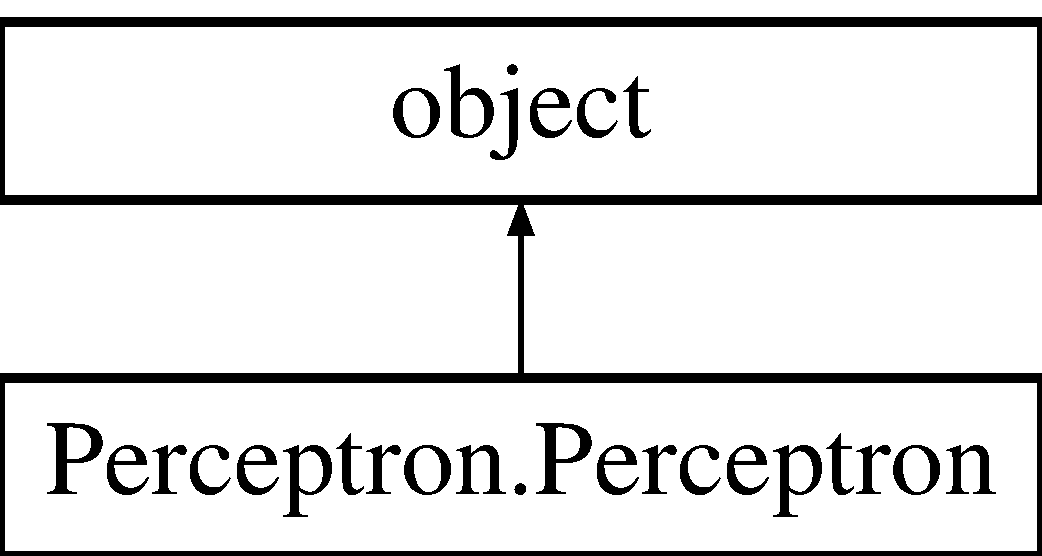
\includegraphics[height=2.000000cm]{class_perceptron_1_1_perceptron}
\end{center}
\end{figure}
\subsection*{Öffentliche Methoden}
\begin{DoxyCompactItemize}
\item 
def \mbox{\hyperlink{class_perceptron_1_1_perceptron_a612d2470864b433455123ab67596c79e}{\+\_\+\+\_\+init\+\_\+\+\_\+}} (self, \mbox{\hyperlink{class_perceptron_1_1_perceptron_a74c50bc1321f3e226ca4e0f96316378d}{eta}}=0.\+01, \mbox{\hyperlink{class_perceptron_1_1_perceptron_a39c8cf01e04f72473ea4b817fbc32405}{n\+\_\+iter}}=50, \mbox{\hyperlink{class_perceptron_1_1_perceptron_ab6afa4dc8b06b17e82885aaf6c20aa81}{random\+\_\+state}}=1)
\item 
def \mbox{\hyperlink{class_perceptron_1_1_perceptron_a2479bd0c6de945508cf00933916bb2a6}{fit}} (self, X, y, w)
\item 
def \mbox{\hyperlink{class_perceptron_1_1_perceptron_a21cab7a11445f766e6258d71529da03f}{net\+\_\+input}} (self, X)
\item 
def \mbox{\hyperlink{class_perceptron_1_1_perceptron_abe5ade4bde9e08101baaec87b53e7b6e}{predict}} (self, X)
\item 
def \mbox{\hyperlink{class_perceptron_1_1_perceptron_a5d312133ac49a2238ef5f06dc0917592}{show\+\_\+tf}} (self, X, y, tf\+\_\+iter=1)
\end{DoxyCompactItemize}
\subsection*{Öffentliche Attribute}
\begin{DoxyCompactItemize}
\item 
\mbox{\hyperlink{class_perceptron_1_1_perceptron_a74c50bc1321f3e226ca4e0f96316378d}{eta}}
\item 
\mbox{\hyperlink{class_perceptron_1_1_perceptron_a39c8cf01e04f72473ea4b817fbc32405}{n\+\_\+iter}}
\item 
\mbox{\hyperlink{class_perceptron_1_1_perceptron_ab6afa4dc8b06b17e82885aaf6c20aa81}{random\+\_\+state}}
\item 
\mbox{\hyperlink{class_perceptron_1_1_perceptron_ae70631ee7d9fbd1c562c9891941d6a62}{w\+\_\+}}
\item 
\mbox{\hyperlink{class_perceptron_1_1_perceptron_af304ae57628fdf47e1d2fec6cc5f5417}{errors\+\_\+}}
\end{DoxyCompactItemize}


\subsection{Ausführliche Beschreibung}
\begin{DoxyVerb}Perceptron classifier.

Parameters
------------
eta : float
  Learning rate (between 0.0 and 1.0)
n_iter : int
  Passes over the training dataset.
random_state : int
  Random number generator seed for random weight
  initialization.

Attributes
-----------
w_ : 1d-array
  Weights after fitting.
errors_ : list
  Number of misclassifications (updates) in each epoch.\end{DoxyVerb}
 

\subsection{Beschreibung der Konstruktoren und Destruktoren}
\mbox{\Hypertarget{class_perceptron_1_1_perceptron_a612d2470864b433455123ab67596c79e}\label{class_perceptron_1_1_perceptron_a612d2470864b433455123ab67596c79e}} 
\index{Perceptron\+::\+Perceptron@{Perceptron\+::\+Perceptron}!\+\_\+\+\_\+init\+\_\+\+\_\+@{\+\_\+\+\_\+init\+\_\+\+\_\+}}
\index{\+\_\+\+\_\+init\+\_\+\+\_\+@{\+\_\+\+\_\+init\+\_\+\+\_\+}!Perceptron\+::\+Perceptron@{Perceptron\+::\+Perceptron}}
\subsubsection{\texorpdfstring{\+\_\+\+\_\+init\+\_\+\+\_\+()}{\_\_init\_\_()}}
{\footnotesize\ttfamily def Perceptron.\+Perceptron.\+\_\+\+\_\+init\+\_\+\+\_\+ (\begin{DoxyParamCaption}\item[{}]{self,  }\item[{}]{eta = {\ttfamily 0.01},  }\item[{}]{n\+\_\+iter = {\ttfamily 50},  }\item[{}]{random\+\_\+state = {\ttfamily 1} }\end{DoxyParamCaption})}



\subsection{Dokumentation der Elementfunktionen}
\mbox{\Hypertarget{class_perceptron_1_1_perceptron_a2479bd0c6de945508cf00933916bb2a6}\label{class_perceptron_1_1_perceptron_a2479bd0c6de945508cf00933916bb2a6}} 
\index{Perceptron\+::\+Perceptron@{Perceptron\+::\+Perceptron}!fit@{fit}}
\index{fit@{fit}!Perceptron\+::\+Perceptron@{Perceptron\+::\+Perceptron}}
\subsubsection{\texorpdfstring{fit()}{fit()}}
{\footnotesize\ttfamily def Perceptron.\+Perceptron.\+fit (\begin{DoxyParamCaption}\item[{}]{self,  }\item[{}]{X,  }\item[{}]{y,  }\item[{}]{w }\end{DoxyParamCaption})}

\begin{DoxyVerb}Fit training data.

Parameters
----------
X : {array-like}, shape = [n_samples, n_features]
  Training vectors, where n_samples is the number of samples and
  n_features is the number of features.
y : array-like, shape = [n_samples]
  Target values.

Returns
-------
self : object\end{DoxyVerb}
 \mbox{\Hypertarget{class_perceptron_1_1_perceptron_a21cab7a11445f766e6258d71529da03f}\label{class_perceptron_1_1_perceptron_a21cab7a11445f766e6258d71529da03f}} 
\index{Perceptron\+::\+Perceptron@{Perceptron\+::\+Perceptron}!net\+\_\+input@{net\+\_\+input}}
\index{net\+\_\+input@{net\+\_\+input}!Perceptron\+::\+Perceptron@{Perceptron\+::\+Perceptron}}
\subsubsection{\texorpdfstring{net\+\_\+input()}{net\_input()}}
{\footnotesize\ttfamily def Perceptron.\+Perceptron.\+net\+\_\+input (\begin{DoxyParamCaption}\item[{}]{self,  }\item[{}]{X }\end{DoxyParamCaption})}

\begin{DoxyVerb}Calculate net input\end{DoxyVerb}
 \mbox{\Hypertarget{class_perceptron_1_1_perceptron_abe5ade4bde9e08101baaec87b53e7b6e}\label{class_perceptron_1_1_perceptron_abe5ade4bde9e08101baaec87b53e7b6e}} 
\index{Perceptron\+::\+Perceptron@{Perceptron\+::\+Perceptron}!predict@{predict}}
\index{predict@{predict}!Perceptron\+::\+Perceptron@{Perceptron\+::\+Perceptron}}
\subsubsection{\texorpdfstring{predict()}{predict()}}
{\footnotesize\ttfamily def Perceptron.\+Perceptron.\+predict (\begin{DoxyParamCaption}\item[{}]{self,  }\item[{}]{X }\end{DoxyParamCaption})}

\begin{DoxyVerb}Return class label after unit step\end{DoxyVerb}
 \mbox{\Hypertarget{class_perceptron_1_1_perceptron_a5d312133ac49a2238ef5f06dc0917592}\label{class_perceptron_1_1_perceptron_a5d312133ac49a2238ef5f06dc0917592}} 
\index{Perceptron\+::\+Perceptron@{Perceptron\+::\+Perceptron}!show\+\_\+tf@{show\+\_\+tf}}
\index{show\+\_\+tf@{show\+\_\+tf}!Perceptron\+::\+Perceptron@{Perceptron\+::\+Perceptron}}
\subsubsection{\texorpdfstring{show\+\_\+tf()}{show\_tf()}}
{\footnotesize\ttfamily def Perceptron.\+Perceptron.\+show\+\_\+tf (\begin{DoxyParamCaption}\item[{}]{self,  }\item[{}]{X,  }\item[{}]{y,  }\item[{}]{tf\+\_\+iter = {\ttfamily 1} }\end{DoxyParamCaption})}



\subsection{Dokumentation der Datenelemente}
\mbox{\Hypertarget{class_perceptron_1_1_perceptron_af304ae57628fdf47e1d2fec6cc5f5417}\label{class_perceptron_1_1_perceptron_af304ae57628fdf47e1d2fec6cc5f5417}} 
\index{Perceptron\+::\+Perceptron@{Perceptron\+::\+Perceptron}!errors\+\_\+@{errors\+\_\+}}
\index{errors\+\_\+@{errors\+\_\+}!Perceptron\+::\+Perceptron@{Perceptron\+::\+Perceptron}}
\subsubsection{\texorpdfstring{errors\+\_\+}{errors\_}}
{\footnotesize\ttfamily Perceptron.\+Perceptron.\+errors\+\_\+}

\mbox{\Hypertarget{class_perceptron_1_1_perceptron_a74c50bc1321f3e226ca4e0f96316378d}\label{class_perceptron_1_1_perceptron_a74c50bc1321f3e226ca4e0f96316378d}} 
\index{Perceptron\+::\+Perceptron@{Perceptron\+::\+Perceptron}!eta@{eta}}
\index{eta@{eta}!Perceptron\+::\+Perceptron@{Perceptron\+::\+Perceptron}}
\subsubsection{\texorpdfstring{eta}{eta}}
{\footnotesize\ttfamily Perceptron.\+Perceptron.\+eta}

\mbox{\Hypertarget{class_perceptron_1_1_perceptron_a39c8cf01e04f72473ea4b817fbc32405}\label{class_perceptron_1_1_perceptron_a39c8cf01e04f72473ea4b817fbc32405}} 
\index{Perceptron\+::\+Perceptron@{Perceptron\+::\+Perceptron}!n\+\_\+iter@{n\+\_\+iter}}
\index{n\+\_\+iter@{n\+\_\+iter}!Perceptron\+::\+Perceptron@{Perceptron\+::\+Perceptron}}
\subsubsection{\texorpdfstring{n\+\_\+iter}{n\_iter}}
{\footnotesize\ttfamily Perceptron.\+Perceptron.\+n\+\_\+iter}

\mbox{\Hypertarget{class_perceptron_1_1_perceptron_ab6afa4dc8b06b17e82885aaf6c20aa81}\label{class_perceptron_1_1_perceptron_ab6afa4dc8b06b17e82885aaf6c20aa81}} 
\index{Perceptron\+::\+Perceptron@{Perceptron\+::\+Perceptron}!random\+\_\+state@{random\+\_\+state}}
\index{random\+\_\+state@{random\+\_\+state}!Perceptron\+::\+Perceptron@{Perceptron\+::\+Perceptron}}
\subsubsection{\texorpdfstring{random\+\_\+state}{random\_state}}
{\footnotesize\ttfamily Perceptron.\+Perceptron.\+random\+\_\+state}

\mbox{\Hypertarget{class_perceptron_1_1_perceptron_ae70631ee7d9fbd1c562c9891941d6a62}\label{class_perceptron_1_1_perceptron_ae70631ee7d9fbd1c562c9891941d6a62}} 
\index{Perceptron\+::\+Perceptron@{Perceptron\+::\+Perceptron}!w\+\_\+@{w\+\_\+}}
\index{w\+\_\+@{w\+\_\+}!Perceptron\+::\+Perceptron@{Perceptron\+::\+Perceptron}}
\subsubsection{\texorpdfstring{w\+\_\+}{w\_}}
{\footnotesize\ttfamily Perceptron.\+Perceptron.\+w\+\_\+}



Die Dokumentation für diese Klasse wurde erzeugt aufgrund der Datei\+:\begin{DoxyCompactItemize}
\item 
C\+:/\+Users/flach/\+Documents/\+Lehre/\+Module/\+T\+S\+V/notebooks/\+L\+V\+\_\+\+T\+S\+V\+\_\+repos/aktuell/functions/\mbox{\hyperlink{_perceptron_8py}{Perceptron.\+py}}\end{DoxyCompactItemize}

\hypertarget{class_pretty_table_1_1_pretty_table}{}\section{Pretty\+Table.\+Pretty\+Table Klassenreferenz}
\label{class_pretty_table_1_1_pretty_table}\index{Pretty\+Table.\+Pretty\+Table@{Pretty\+Table.\+Pretty\+Table}}
Klassendiagramm für Pretty\+Table.\+Pretty\+Table\+:\begin{figure}[H]
\begin{center}
\leavevmode
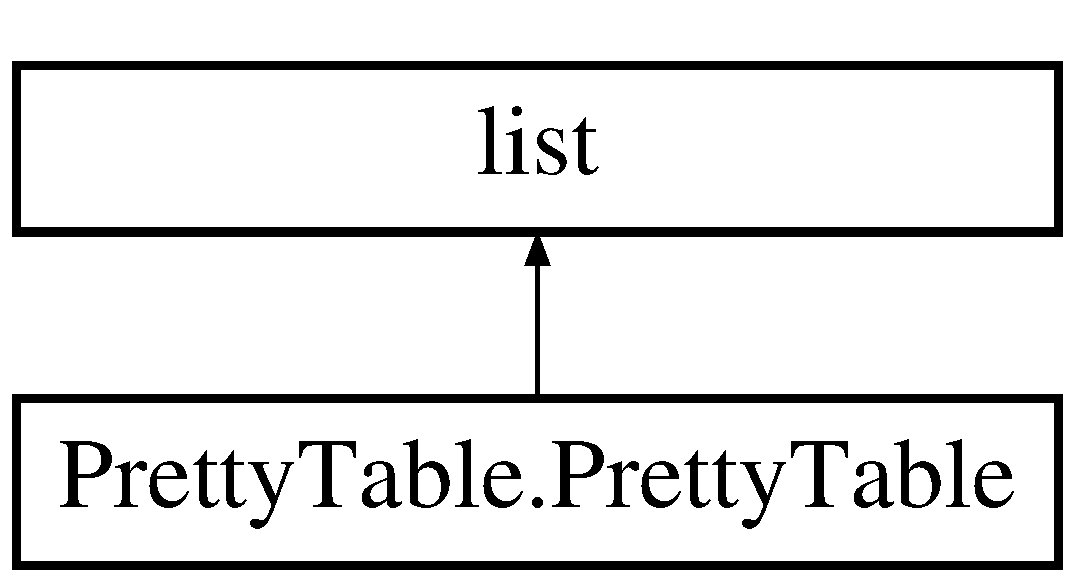
\includegraphics[height=2.000000cm]{class_pretty_table_1_1_pretty_table}
\end{center}
\end{figure}
\subsection*{Öffentliche Methoden}
\begin{DoxyCompactItemize}
\item 
def \mbox{\hyperlink{class_pretty_table_1_1_pretty_table_ab55e014c286d85c331f9df095008a6a2}{\+\_\+\+\_\+init\+\_\+\+\_\+}} (self, initlist=\mbox{[}$\,$\mbox{]}, extra\+\_\+header=None, \mbox{\hyperlink{class_pretty_table_1_1_pretty_table_a871a7b01d3f42d1a0e053a2cd1a98dbc}{print\+\_\+latex\+\_\+longtable}}=True)
\item 
def \mbox{\hyperlink{class_pretty_table_1_1_pretty_table_a47ca8c24fce0d42d04f689931f01ba3a}{latex\+\_\+table\+\_\+tabular}} (self)
\item 
def \mbox{\hyperlink{class_pretty_table_1_1_pretty_table_a2a1c5a4e3ffdd78cb58b17c492a9da39}{latex\+\_\+longtable}} (self)
\end{DoxyCompactItemize}
\subsection*{Öffentliche Attribute}
\begin{DoxyCompactItemize}
\item 
\mbox{\hyperlink{class_pretty_table_1_1_pretty_table_a871a7b01d3f42d1a0e053a2cd1a98dbc}{print\+\_\+latex\+\_\+longtable}}
\end{DoxyCompactItemize}


\subsection{Ausführliche Beschreibung}
\begin{DoxyVerb}Overridden list class which takes a 2-dimensional list of 
    the form [[1,2,3],[4,5,6]], and renders HTML and LaTeX Table in 
    IPython Notebook. For LaTeX export two styles can be chosen.\end{DoxyVerb}
 

\subsection{Beschreibung der Konstruktoren und Destruktoren}
\mbox{\Hypertarget{class_pretty_table_1_1_pretty_table_ab55e014c286d85c331f9df095008a6a2}\label{class_pretty_table_1_1_pretty_table_ab55e014c286d85c331f9df095008a6a2}} 
\index{Pretty\+Table\+::\+Pretty\+Table@{Pretty\+Table\+::\+Pretty\+Table}!\+\_\+\+\_\+init\+\_\+\+\_\+@{\+\_\+\+\_\+init\+\_\+\+\_\+}}
\index{\+\_\+\+\_\+init\+\_\+\+\_\+@{\+\_\+\+\_\+init\+\_\+\+\_\+}!Pretty\+Table\+::\+Pretty\+Table@{Pretty\+Table\+::\+Pretty\+Table}}
\subsubsection{\texorpdfstring{\+\_\+\+\_\+init\+\_\+\+\_\+()}{\_\_init\_\_()}}
{\footnotesize\ttfamily def Pretty\+Table.\+Pretty\+Table.\+\_\+\+\_\+init\+\_\+\+\_\+ (\begin{DoxyParamCaption}\item[{}]{self,  }\item[{}]{initlist = {\ttfamily \mbox{[}\mbox{]}},  }\item[{}]{extra\+\_\+header = {\ttfamily None},  }\item[{}]{print\+\_\+latex\+\_\+longtable = {\ttfamily True} }\end{DoxyParamCaption})}



\subsection{Dokumentation der Elementfunktionen}
\mbox{\Hypertarget{class_pretty_table_1_1_pretty_table_a2a1c5a4e3ffdd78cb58b17c492a9da39}\label{class_pretty_table_1_1_pretty_table_a2a1c5a4e3ffdd78cb58b17c492a9da39}} 
\index{Pretty\+Table\+::\+Pretty\+Table@{Pretty\+Table\+::\+Pretty\+Table}!latex\+\_\+longtable@{latex\+\_\+longtable}}
\index{latex\+\_\+longtable@{latex\+\_\+longtable}!Pretty\+Table\+::\+Pretty\+Table@{Pretty\+Table\+::\+Pretty\+Table}}
\subsubsection{\texorpdfstring{latex\+\_\+longtable()}{latex\_longtable()}}
{\footnotesize\ttfamily def Pretty\+Table.\+Pretty\+Table.\+latex\+\_\+longtable (\begin{DoxyParamCaption}\item[{}]{self }\end{DoxyParamCaption})}

\mbox{\Hypertarget{class_pretty_table_1_1_pretty_table_a47ca8c24fce0d42d04f689931f01ba3a}\label{class_pretty_table_1_1_pretty_table_a47ca8c24fce0d42d04f689931f01ba3a}} 
\index{Pretty\+Table\+::\+Pretty\+Table@{Pretty\+Table\+::\+Pretty\+Table}!latex\+\_\+table\+\_\+tabular@{latex\+\_\+table\+\_\+tabular}}
\index{latex\+\_\+table\+\_\+tabular@{latex\+\_\+table\+\_\+tabular}!Pretty\+Table\+::\+Pretty\+Table@{Pretty\+Table\+::\+Pretty\+Table}}
\subsubsection{\texorpdfstring{latex\+\_\+table\+\_\+tabular()}{latex\_table\_tabular()}}
{\footnotesize\ttfamily def Pretty\+Table.\+Pretty\+Table.\+latex\+\_\+table\+\_\+tabular (\begin{DoxyParamCaption}\item[{}]{self }\end{DoxyParamCaption})}



\subsection{Dokumentation der Datenelemente}
\mbox{\Hypertarget{class_pretty_table_1_1_pretty_table_a871a7b01d3f42d1a0e053a2cd1a98dbc}\label{class_pretty_table_1_1_pretty_table_a871a7b01d3f42d1a0e053a2cd1a98dbc}} 
\index{Pretty\+Table\+::\+Pretty\+Table@{Pretty\+Table\+::\+Pretty\+Table}!print\+\_\+latex\+\_\+longtable@{print\+\_\+latex\+\_\+longtable}}
\index{print\+\_\+latex\+\_\+longtable@{print\+\_\+latex\+\_\+longtable}!Pretty\+Table\+::\+Pretty\+Table@{Pretty\+Table\+::\+Pretty\+Table}}
\subsubsection{\texorpdfstring{print\+\_\+latex\+\_\+longtable}{print\_latex\_longtable}}
{\footnotesize\ttfamily Pretty\+Table.\+Pretty\+Table.\+print\+\_\+latex\+\_\+longtable}



Die Dokumentation für diese Klasse wurde erzeugt aufgrund der Datei\+:\begin{DoxyCompactItemize}
\item 
C\+:/\+Users/flach/\+Documents/\+Lehre/\+Module/\+T\+S\+V/notebooks/\+L\+V\+\_\+\+T\+S\+V\+\_\+repos/aktuell/functions/\mbox{\hyperlink{_pretty_table_8py}{Pretty\+Table.\+py}}\end{DoxyCompactItemize}

\hypertarget{classsounddata_1_1_sounddata}{}\section{sounddata.\+Sounddata Klassenreferenz}
\label{classsounddata_1_1_sounddata}\index{sounddata.\+Sounddata@{sounddata.\+Sounddata}}


Dokumentation für die Klasse \mbox{\hyperlink{classsounddata_1_1_sounddata}{Sounddata}}.  


\subsection*{Öffentliche Methoden}
\begin{DoxyCompactItemize}
\item 
def \mbox{\hyperlink{classsounddata_1_1_sounddata_a5bd8d7eebdf0bb0d137bfeb74b4c9fe6}{\+\_\+\+\_\+init\+\_\+\+\_\+}} (self, fn, vs=\textquotesingle{}\textquotesingle{}, fs=44000, df=\textquotesingle{}\textquotesingle{}, atw=0, sd\+\_\+min=0, sd\+\_\+max=0, \mbox{\hyperlink{classsounddata_1_1_sounddata_a64a625b1f08e5888cd34e14aad188cc0}{data}}=\mbox{[}$\,$\mbox{]})
\item 
def \mbox{\hyperlink{classsounddata_1_1_sounddata_a198de54d49c935b70cf8545980af1c26}{set\+\_\+info}} (self)
\begin{DoxyCompactList}\small\item\em setzt für angegebenes Soundobjekt die Attributwerte \end{DoxyCompactList}\item 
def \mbox{\hyperlink{classsounddata_1_1_sounddata_ac63cbec499bc5b28eced6ff6d0187376}{get\+\_\+info}} (self, attr)
\begin{DoxyCompactList}\small\item\em ermittelt für angegebenes Soundobjekt Wert des Attributes, wenn leer, dann alle Attribute \end{DoxyCompactList}\item 
def \mbox{\hyperlink{classsounddata_1_1_sounddata_a88a9e2052bdaa80e988bb0d4f5610495}{read\+\_\+sound}} (self)
\begin{DoxyCompactList}\small\item\em liest Daten in Soundobjekt ein \end{DoxyCompactList}\item 
def \mbox{\hyperlink{classsounddata_1_1_sounddata_abcf4edd6915714cc4db89ab787ab4007}{write\+\_\+sound}} (self)
\begin{DoxyCompactList}\small\item\em schreibt Daten des Soundobjektes \end{DoxyCompactList}\item 
def \mbox{\hyperlink{classsounddata_1_1_sounddata_a623c2b2a5e126347893864ffc09246d6}{normalize\+\_\+sound}} (self)
\begin{DoxyCompactList}\small\item\em normiert Soundobjekt \end{DoxyCompactList}\item 
def \mbox{\hyperlink{classsounddata_1_1_sounddata_aacf5b956e13132ce48a550852b6e9a96}{play\+\_\+sound}} (self)
\begin{DoxyCompactList}\small\item\em gibt Soundobjekt wieder \end{DoxyCompactList}\end{DoxyCompactItemize}
\subsection*{Öffentliche Attribute}
\begin{DoxyCompactItemize}
\item 
\mbox{\hyperlink{classsounddata_1_1_sounddata_ab95569d979168deb16d06ddfdb838603}{Filename}}
\begin{DoxyCompactList}\small\item\em Filename. \end{DoxyCompactList}\item 
\mbox{\hyperlink{classsounddata_1_1_sounddata_a9a4ef06c4e02480837e12b98e1e75bfe}{Verschriftung}}
\begin{DoxyCompactList}\small\item\em Verschriftung der Sprachäußerung. \end{DoxyCompactList}\item 
\mbox{\hyperlink{classsounddata_1_1_sounddata_a1519ee17817b6a2c9107ca5e5d09f204}{Abtastfrequenz}}
\begin{DoxyCompactList}\small\item\em Abtastfrequenz in Hz. \end{DoxyCompactList}\item 
\mbox{\hyperlink{classsounddata_1_1_sounddata_ada2e26b302a4e72ce4a77858510032eb}{Datenformat}}
\begin{DoxyCompactList}\small\item\em Datenformat. \end{DoxyCompactList}\item 
\mbox{\hyperlink{classsounddata_1_1_sounddata_afe517ca7dfaa55c4418966f98063dda8}{A\+TW}}
\begin{DoxyCompactList}\small\item\em Anzahl Abtastwerte. \end{DoxyCompactList}\item 
\mbox{\hyperlink{classsounddata_1_1_sounddata_a57cdccd0a2cae0a3f39b7a40a6f1d5f8}{min}}
\begin{DoxyCompactList}\small\item\em kleinster Abtastwert \end{DoxyCompactList}\item 
\mbox{\hyperlink{classsounddata_1_1_sounddata_a9d4467c1e463d7edacf1d4f540d0f3d1}{max}}
\begin{DoxyCompactList}\small\item\em größter Abtastwert \end{DoxyCompactList}\item 
\mbox{\hyperlink{classsounddata_1_1_sounddata_a64a625b1f08e5888cd34e14aad188cc0}{data}}
\begin{DoxyCompactList}\small\item\em Datenfeld. \end{DoxyCompactList}\end{DoxyCompactItemize}


\subsection{Ausführliche Beschreibung}
Dokumentation für die Klasse \mbox{\hyperlink{classsounddata_1_1_sounddata}{Sounddata}}. 

Handling von Sounddaten

Zur Beschreibung der Objekte werden folgende Attribute verwendet\+: ~\newline
 Filename; Verschriftung; Abtastfrequenz; Datenformat; Anz. Abtastwerte; Minumum; Maximum

Folgende Methoden stehen zur Verfügung\+: \mbox{\hyperlink{classsounddata_1_1_sounddata_a198de54d49c935b70cf8545980af1c26}{set\+\_\+info()}}; \mbox{\hyperlink{classsounddata_1_1_sounddata_ac63cbec499bc5b28eced6ff6d0187376}{get\+\_\+info()}}; \mbox{\hyperlink{classsounddata_1_1_sounddata_a88a9e2052bdaa80e988bb0d4f5610495}{read\+\_\+sound()}}; \mbox{\hyperlink{classsounddata_1_1_sounddata_abcf4edd6915714cc4db89ab787ab4007}{write\+\_\+sound()}}; \mbox{\hyperlink{classsounddata_1_1_sounddata_a623c2b2a5e126347893864ffc09246d6}{normalize\+\_\+sound()}};\mbox{\hyperlink{classsounddata_1_1_sounddata_aacf5b956e13132ce48a550852b6e9a96}{play\+\_\+sound()}}. 

\subsection{Beschreibung der Konstruktoren und Destruktoren}
\mbox{\Hypertarget{classsounddata_1_1_sounddata_a5bd8d7eebdf0bb0d137bfeb74b4c9fe6}\label{classsounddata_1_1_sounddata_a5bd8d7eebdf0bb0d137bfeb74b4c9fe6}} 
\index{sounddata\+::\+Sounddata@{sounddata\+::\+Sounddata}!\+\_\+\+\_\+init\+\_\+\+\_\+@{\+\_\+\+\_\+init\+\_\+\+\_\+}}
\index{\+\_\+\+\_\+init\+\_\+\+\_\+@{\+\_\+\+\_\+init\+\_\+\+\_\+}!sounddata\+::\+Sounddata@{sounddata\+::\+Sounddata}}
\subsubsection{\texorpdfstring{\+\_\+\+\_\+init\+\_\+\+\_\+()}{\_\_init\_\_()}}
{\footnotesize\ttfamily def sounddata.\+Sounddata.\+\_\+\+\_\+init\+\_\+\+\_\+ (\begin{DoxyParamCaption}\item[{}]{self,  }\item[{}]{fn,  }\item[{}]{vs = {\ttfamily \textquotesingle{}\textquotesingle{}},  }\item[{}]{fs = {\ttfamily 44000},  }\item[{}]{df = {\ttfamily \textquotesingle{}\textquotesingle{}},  }\item[{}]{atw = {\ttfamily 0},  }\item[{}]{sd\+\_\+min = {\ttfamily 0},  }\item[{}]{sd\+\_\+max = {\ttfamily 0},  }\item[{}]{data = {\ttfamily \mbox{[}\mbox{]}} }\end{DoxyParamCaption})}



\subsection{Dokumentation der Elementfunktionen}
\mbox{\Hypertarget{classsounddata_1_1_sounddata_ac63cbec499bc5b28eced6ff6d0187376}\label{classsounddata_1_1_sounddata_ac63cbec499bc5b28eced6ff6d0187376}} 
\index{sounddata\+::\+Sounddata@{sounddata\+::\+Sounddata}!get\+\_\+info@{get\+\_\+info}}
\index{get\+\_\+info@{get\+\_\+info}!sounddata\+::\+Sounddata@{sounddata\+::\+Sounddata}}
\subsubsection{\texorpdfstring{get\+\_\+info()}{get\_info()}}
{\footnotesize\ttfamily def sounddata.\+Sounddata.\+get\+\_\+info (\begin{DoxyParamCaption}\item[{}]{self,  }\item[{}]{attr }\end{DoxyParamCaption})}



ermittelt für angegebenes Soundobjekt Wert des Attributes, wenn leer, dann alle Attribute 


\begin{DoxyParams}{Parameter}
{\em self} & Objektzeiger \\
\hline
{\em attr} & gewünschtes Attribut \\
\hline
\end{DoxyParams}
\mbox{\Hypertarget{classsounddata_1_1_sounddata_a623c2b2a5e126347893864ffc09246d6}\label{classsounddata_1_1_sounddata_a623c2b2a5e126347893864ffc09246d6}} 
\index{sounddata\+::\+Sounddata@{sounddata\+::\+Sounddata}!normalize\+\_\+sound@{normalize\+\_\+sound}}
\index{normalize\+\_\+sound@{normalize\+\_\+sound}!sounddata\+::\+Sounddata@{sounddata\+::\+Sounddata}}
\subsubsection{\texorpdfstring{normalize\+\_\+sound()}{normalize\_sound()}}
{\footnotesize\ttfamily def sounddata.\+Sounddata.\+normalize\+\_\+sound (\begin{DoxyParamCaption}\item[{}]{self }\end{DoxyParamCaption})}



normiert Soundobjekt 


\begin{DoxyParams}{Parameter}
{\em self} & Objektzeiger \\
\hline
\end{DoxyParams}
\mbox{\Hypertarget{classsounddata_1_1_sounddata_aacf5b956e13132ce48a550852b6e9a96}\label{classsounddata_1_1_sounddata_aacf5b956e13132ce48a550852b6e9a96}} 
\index{sounddata\+::\+Sounddata@{sounddata\+::\+Sounddata}!play\+\_\+sound@{play\+\_\+sound}}
\index{play\+\_\+sound@{play\+\_\+sound}!sounddata\+::\+Sounddata@{sounddata\+::\+Sounddata}}
\subsubsection{\texorpdfstring{play\+\_\+sound()}{play\_sound()}}
{\footnotesize\ttfamily def sounddata.\+Sounddata.\+play\+\_\+sound (\begin{DoxyParamCaption}\item[{}]{self }\end{DoxyParamCaption})}



gibt Soundobjekt wieder 


\begin{DoxyParams}{Parameter}
{\em self} & Objektzeiger \\
\hline
\end{DoxyParams}
\mbox{\Hypertarget{classsounddata_1_1_sounddata_a88a9e2052bdaa80e988bb0d4f5610495}\label{classsounddata_1_1_sounddata_a88a9e2052bdaa80e988bb0d4f5610495}} 
\index{sounddata\+::\+Sounddata@{sounddata\+::\+Sounddata}!read\+\_\+sound@{read\+\_\+sound}}
\index{read\+\_\+sound@{read\+\_\+sound}!sounddata\+::\+Sounddata@{sounddata\+::\+Sounddata}}
\subsubsection{\texorpdfstring{read\+\_\+sound()}{read\_sound()}}
{\footnotesize\ttfamily def sounddata.\+Sounddata.\+read\+\_\+sound (\begin{DoxyParamCaption}\item[{}]{self }\end{DoxyParamCaption})}



liest Daten in Soundobjekt ein 


\begin{DoxyParams}{Parameter}
{\em self} & Objektzeiger \\
\hline
\end{DoxyParams}
\mbox{\Hypertarget{classsounddata_1_1_sounddata_a198de54d49c935b70cf8545980af1c26}\label{classsounddata_1_1_sounddata_a198de54d49c935b70cf8545980af1c26}} 
\index{sounddata\+::\+Sounddata@{sounddata\+::\+Sounddata}!set\+\_\+info@{set\+\_\+info}}
\index{set\+\_\+info@{set\+\_\+info}!sounddata\+::\+Sounddata@{sounddata\+::\+Sounddata}}
\subsubsection{\texorpdfstring{set\+\_\+info()}{set\_info()}}
{\footnotesize\ttfamily def sounddata.\+Sounddata.\+set\+\_\+info (\begin{DoxyParamCaption}\item[{}]{self }\end{DoxyParamCaption})}



setzt für angegebenes Soundobjekt die Attributwerte 


\begin{DoxyParams}{Parameter}
{\em self} & Objektzeiger \\
\hline
\end{DoxyParams}
\mbox{\Hypertarget{classsounddata_1_1_sounddata_abcf4edd6915714cc4db89ab787ab4007}\label{classsounddata_1_1_sounddata_abcf4edd6915714cc4db89ab787ab4007}} 
\index{sounddata\+::\+Sounddata@{sounddata\+::\+Sounddata}!write\+\_\+sound@{write\+\_\+sound}}
\index{write\+\_\+sound@{write\+\_\+sound}!sounddata\+::\+Sounddata@{sounddata\+::\+Sounddata}}
\subsubsection{\texorpdfstring{write\+\_\+sound()}{write\_sound()}}
{\footnotesize\ttfamily def sounddata.\+Sounddata.\+write\+\_\+sound (\begin{DoxyParamCaption}\item[{}]{self }\end{DoxyParamCaption})}



schreibt Daten des Soundobjektes 


\begin{DoxyParams}{Parameter}
{\em self} & Objektzeiger \\
\hline
\end{DoxyParams}


\subsection{Dokumentation der Datenelemente}
\mbox{\Hypertarget{classsounddata_1_1_sounddata_a1519ee17817b6a2c9107ca5e5d09f204}\label{classsounddata_1_1_sounddata_a1519ee17817b6a2c9107ca5e5d09f204}} 
\index{sounddata\+::\+Sounddata@{sounddata\+::\+Sounddata}!Abtastfrequenz@{Abtastfrequenz}}
\index{Abtastfrequenz@{Abtastfrequenz}!sounddata\+::\+Sounddata@{sounddata\+::\+Sounddata}}
\subsubsection{\texorpdfstring{Abtastfrequenz}{Abtastfrequenz}}
{\footnotesize\ttfamily sounddata.\+Sounddata.\+Abtastfrequenz}



Abtastfrequenz in Hz. 

\mbox{\Hypertarget{classsounddata_1_1_sounddata_afe517ca7dfaa55c4418966f98063dda8}\label{classsounddata_1_1_sounddata_afe517ca7dfaa55c4418966f98063dda8}} 
\index{sounddata\+::\+Sounddata@{sounddata\+::\+Sounddata}!A\+TW@{A\+TW}}
\index{A\+TW@{A\+TW}!sounddata\+::\+Sounddata@{sounddata\+::\+Sounddata}}
\subsubsection{\texorpdfstring{A\+TW}{ATW}}
{\footnotesize\ttfamily sounddata.\+Sounddata.\+A\+TW}



Anzahl Abtastwerte. 

\mbox{\Hypertarget{classsounddata_1_1_sounddata_a64a625b1f08e5888cd34e14aad188cc0}\label{classsounddata_1_1_sounddata_a64a625b1f08e5888cd34e14aad188cc0}} 
\index{sounddata\+::\+Sounddata@{sounddata\+::\+Sounddata}!data@{data}}
\index{data@{data}!sounddata\+::\+Sounddata@{sounddata\+::\+Sounddata}}
\subsubsection{\texorpdfstring{data}{data}}
{\footnotesize\ttfamily sounddata.\+Sounddata.\+data}



Datenfeld. 

\mbox{\Hypertarget{classsounddata_1_1_sounddata_ada2e26b302a4e72ce4a77858510032eb}\label{classsounddata_1_1_sounddata_ada2e26b302a4e72ce4a77858510032eb}} 
\index{sounddata\+::\+Sounddata@{sounddata\+::\+Sounddata}!Datenformat@{Datenformat}}
\index{Datenformat@{Datenformat}!sounddata\+::\+Sounddata@{sounddata\+::\+Sounddata}}
\subsubsection{\texorpdfstring{Datenformat}{Datenformat}}
{\footnotesize\ttfamily sounddata.\+Sounddata.\+Datenformat}



Datenformat. 

\mbox{\Hypertarget{classsounddata_1_1_sounddata_ab95569d979168deb16d06ddfdb838603}\label{classsounddata_1_1_sounddata_ab95569d979168deb16d06ddfdb838603}} 
\index{sounddata\+::\+Sounddata@{sounddata\+::\+Sounddata}!Filename@{Filename}}
\index{Filename@{Filename}!sounddata\+::\+Sounddata@{sounddata\+::\+Sounddata}}
\subsubsection{\texorpdfstring{Filename}{Filename}}
{\footnotesize\ttfamily sounddata.\+Sounddata.\+Filename}



Filename. 

\mbox{\Hypertarget{classsounddata_1_1_sounddata_a9d4467c1e463d7edacf1d4f540d0f3d1}\label{classsounddata_1_1_sounddata_a9d4467c1e463d7edacf1d4f540d0f3d1}} 
\index{sounddata\+::\+Sounddata@{sounddata\+::\+Sounddata}!max@{max}}
\index{max@{max}!sounddata\+::\+Sounddata@{sounddata\+::\+Sounddata}}
\subsubsection{\texorpdfstring{max}{max}}
{\footnotesize\ttfamily sounddata.\+Sounddata.\+max}



größter Abtastwert 

\mbox{\Hypertarget{classsounddata_1_1_sounddata_a57cdccd0a2cae0a3f39b7a40a6f1d5f8}\label{classsounddata_1_1_sounddata_a57cdccd0a2cae0a3f39b7a40a6f1d5f8}} 
\index{sounddata\+::\+Sounddata@{sounddata\+::\+Sounddata}!min@{min}}
\index{min@{min}!sounddata\+::\+Sounddata@{sounddata\+::\+Sounddata}}
\subsubsection{\texorpdfstring{min}{min}}
{\footnotesize\ttfamily sounddata.\+Sounddata.\+min}



kleinster Abtastwert 

\mbox{\Hypertarget{classsounddata_1_1_sounddata_a9a4ef06c4e02480837e12b98e1e75bfe}\label{classsounddata_1_1_sounddata_a9a4ef06c4e02480837e12b98e1e75bfe}} 
\index{sounddata\+::\+Sounddata@{sounddata\+::\+Sounddata}!Verschriftung@{Verschriftung}}
\index{Verschriftung@{Verschriftung}!sounddata\+::\+Sounddata@{sounddata\+::\+Sounddata}}
\subsubsection{\texorpdfstring{Verschriftung}{Verschriftung}}
{\footnotesize\ttfamily sounddata.\+Sounddata.\+Verschriftung}



Verschriftung der Sprachäußerung. 



Die Dokumentation für diese Klasse wurde erzeugt aufgrund der Datei\+:\begin{DoxyCompactItemize}
\item 
C\+:/\+Users/flach/\+Documents/\+Lehre/\+Module/\+T\+S\+V/notebooks/\+L\+V\+\_\+\+T\+S\+V\+\_\+repos/aktuell/functions/\mbox{\hyperlink{sounddata_8py}{sounddata.\+py}}\end{DoxyCompactItemize}

\chapter{Datei-\/\+Dokumentation}
\hypertarget{cepstrum_8py}{}\section{C\+:/\+Users/flach/\+Documents/\+Lehre/\+Module/\+T\+S\+V/notebooks/\+L\+V\+\_\+\+T\+S\+V\+\_\+repos/aktuell/functions/cepstrum.py-\/\+Dateireferenz}
\label{cepstrum_8py}\index{C\+:/\+Users/flach/\+Documents/\+Lehre/\+Module/\+T\+S\+V/notebooks/\+L\+V\+\_\+\+T\+S\+V\+\_\+repos/aktuell/functions/cepstrum.\+py@{C\+:/\+Users/flach/\+Documents/\+Lehre/\+Module/\+T\+S\+V/notebooks/\+L\+V\+\_\+\+T\+S\+V\+\_\+repos/aktuell/functions/cepstrum.\+py}}
\subsection*{Namensbereiche}
\begin{DoxyCompactItemize}
\item 
 \mbox{\hyperlink{namespacecepstrum}{cepstrum}}
\end{DoxyCompactItemize}
\subsection*{Funktionen}
\begin{DoxyCompactItemize}
\item 
def \mbox{\hyperlink{namespacecepstrum_af44fa6a9e5f5e8db043cb60b38894085}{cepstrum.\+read\+\_\+show\+\_\+sig}} (file\+\_\+name, sig\+\_\+dur)
\item 
def \mbox{\hyperlink{namespacecepstrum_ae9a55612bcfeaa372d11036a16b98527}{cepstrum.\+show\+\_\+sig}} (signal, sig\+\_\+dur, file\+\_\+name)
\item 
def \mbox{\hyperlink{namespacecepstrum_ab6397c51bd13894929df2b4c206fecfa}{cepstrum.\+wind\+\_\+sig}} (frame\+\_\+size, frame\+\_\+stride, sample\+\_\+rate, signal)
\item 
def \mbox{\hyperlink{namespacecepstrum_a3db8285f132510ae674c893a651ca971}{cepstrum.\+show\+\_\+spectrogram}} (frames, sig\+\_\+dur, sample\+\_\+rate)
\item 
def \mbox{\hyperlink{namespacecepstrum_ae0a1b2c79db9e80e8dfe58fd9dfb9ad6}{cepstrum.\+mel\+\_\+spec}} (nfilt, sample\+\_\+rate, N\+F\+FT, sig\+\_\+frames)
\item 
def \mbox{\hyperlink{namespacecepstrum_a3e21b1c622287001e82e62c0c64d0643}{cepstrum.\+show\+\_\+melspec}} (mel\+\_\+frames, sig\+\_\+dur, nfilt)
\item 
def \mbox{\hyperlink{namespacecepstrum_a43917229e1efedf7a3439fdfc6b2890a}{cepstrum.\+show\+\_\+mfcc}} (mfcc, sig\+\_\+dur, num\+\_\+ceps)
\end{DoxyCompactItemize}

\hypertarget{_perceptron_8py}{}\section{C\+:/\+Users/flach/\+Documents/\+Lehre/\+Module/\+T\+S\+V/notebooks/\+L\+V\+\_\+\+T\+S\+V\+\_\+repos/aktuell/functions/\+Perceptron.py-\/\+Dateireferenz}
\label{_perceptron_8py}\index{C\+:/\+Users/flach/\+Documents/\+Lehre/\+Module/\+T\+S\+V/notebooks/\+L\+V\+\_\+\+T\+S\+V\+\_\+repos/aktuell/functions/\+Perceptron.\+py@{C\+:/\+Users/flach/\+Documents/\+Lehre/\+Module/\+T\+S\+V/notebooks/\+L\+V\+\_\+\+T\+S\+V\+\_\+repos/aktuell/functions/\+Perceptron.\+py}}
\subsection*{Klassen}
\begin{DoxyCompactItemize}
\item 
class \mbox{\hyperlink{class_perceptron_1_1_perceptron}{Perceptron.\+Perceptron}}
\end{DoxyCompactItemize}
\subsection*{Namensbereiche}
\begin{DoxyCompactItemize}
\item 
 \mbox{\hyperlink{namespace_perceptron}{Perceptron}}
\end{DoxyCompactItemize}

\hypertarget{_pretty_table_8py}{}\section{C\+:/\+Users/flach/\+Documents/\+Lehre/\+Module/\+T\+S\+V/notebooks/\+L\+V\+\_\+\+T\+S\+V\+\_\+repos/aktuell/functions/\+Pretty\+Table.py-\/\+Dateireferenz}
\label{_pretty_table_8py}\index{C\+:/\+Users/flach/\+Documents/\+Lehre/\+Module/\+T\+S\+V/notebooks/\+L\+V\+\_\+\+T\+S\+V\+\_\+repos/aktuell/functions/\+Pretty\+Table.\+py@{C\+:/\+Users/flach/\+Documents/\+Lehre/\+Module/\+T\+S\+V/notebooks/\+L\+V\+\_\+\+T\+S\+V\+\_\+repos/aktuell/functions/\+Pretty\+Table.\+py}}
\subsection*{Klassen}
\begin{DoxyCompactItemize}
\item 
class \mbox{\hyperlink{class_pretty_table_1_1_pretty_table}{Pretty\+Table.\+Pretty\+Table}}
\end{DoxyCompactItemize}
\subsection*{Namensbereiche}
\begin{DoxyCompactItemize}
\item 
 \mbox{\hyperlink{namespace_pretty_table}{Pretty\+Table}}
\end{DoxyCompactItemize}

\hypertarget{print_8py}{}\section{C\+:/\+Users/flach/\+Documents/\+Lehre/\+Module/\+T\+S\+V/notebooks/\+L\+V\+\_\+\+T\+S\+V\+\_\+repos/aktuell/functions/print.py-\/\+Dateireferenz}
\label{print_8py}\index{C\+:/\+Users/flach/\+Documents/\+Lehre/\+Module/\+T\+S\+V/notebooks/\+L\+V\+\_\+\+T\+S\+V\+\_\+repos/aktuell/functions/print.\+py@{C\+:/\+Users/flach/\+Documents/\+Lehre/\+Module/\+T\+S\+V/notebooks/\+L\+V\+\_\+\+T\+S\+V\+\_\+repos/aktuell/functions/print.\+py}}
\subsection*{Namensbereiche}
\begin{DoxyCompactItemize}
\item 
 \mbox{\hyperlink{namespaceprint}{print}}
\end{DoxyCompactItemize}
\subsection*{Variablen}
\begin{DoxyCompactItemize}
\item 
\mbox{\hyperlink{namespaceprint_a8080002122fd53cadd2b548837d037aa}{print.\+fig}} = plt.\+figure(figsize=(10,10))
\item 
\mbox{\hyperlink{namespaceprint_a980229015cfaa5dda779f5e1df7e4013}{print.\+ax}} = fig.\+add\+\_\+subplot(1, 1, 1, projection=\textquotesingle{}3d\textquotesingle{})
\item 
\mbox{\hyperlink{namespaceprint_affd04964e07d6931f5b7f92164b9b99f}{print.\+X}} = np.\+arange(-\/10, 10, 0.\+25)
\item 
\mbox{\hyperlink{namespaceprint_aab512732eb82cbe258baa68f9f9add63}{print.\+Y}} = np.\+arange(-\/10, 10, 0.\+25)
\item 
int \mbox{\hyperlink{namespaceprint_a0d1f4b3564b3a18949e4a9d42c0fe83b}{print.\+mu}} = -\/2
\item 
float \mbox{\hyperlink{namespaceprint_a1efc77cd3bf0d758b07ec8e2b2c71c6b}{print.\+sig}} = 1.\+5
\item 
int \mbox{\hyperlink{namespaceprint_acc02b068ba7893cb51896817458953b1}{print.\+Z1}} = 1/(sig$\ast$np.\+sqrt(2$\ast$np.\+pi))$\ast$np.\+exp(-\/(X -\/ mu)$\ast$$\ast$2/(2$\ast$sig$\ast$$\ast$2))$\ast$\textbackslash{}
\item 
int \mbox{\hyperlink{namespaceprint_a09064592a1be5db47dee477a81ae8bf3}{print.\+Z2}} = 1/(sig$\ast$np.\+sqrt(2$\ast$np.\+pi))$\ast$np.\+exp(-\/(X -\/ mu)$\ast$$\ast$2/(2$\ast$sig$\ast$$\ast$2))$\ast$\textbackslash{}
\item 
int \mbox{\hyperlink{namespaceprint_a9433aedd977f6182d23edaf955e46742}{print.\+Z}} = 4$\ast$Z1 + 5$\ast$Z2
\item 
\mbox{\hyperlink{namespaceprint_a25485f663d582df21114be2f03bad0e0}{print.\+zdir}}
\item 
\mbox{\hyperlink{namespaceprint_a63b63e4e6ea6a9b03c0e161424d919e8}{print.\+offset}}
\item 
\mbox{\hyperlink{namespaceprint_a811f3257310281e4a58230ebd65dcc71}{print.\+levels}}
\item 
\mbox{\hyperlink{namespaceprint_a4c39ba09ea1a62ecd2fc116b9ef27c42}{print.\+cmap}}
\end{DoxyCompactItemize}

\hypertarget{sda__help_8py}{}\section{C\+:/\+Users/flach/\+Documents/\+Lehre/\+Module/\+T\+S\+V/notebooks/\+L\+V\+\_\+\+T\+S\+V\+\_\+repos/aktuell/functions/sda\+\_\+help.py-\/\+Dateireferenz}
\label{sda__help_8py}\index{C\+:/\+Users/flach/\+Documents/\+Lehre/\+Module/\+T\+S\+V/notebooks/\+L\+V\+\_\+\+T\+S\+V\+\_\+repos/aktuell/functions/sda\+\_\+help.\+py@{C\+:/\+Users/flach/\+Documents/\+Lehre/\+Module/\+T\+S\+V/notebooks/\+L\+V\+\_\+\+T\+S\+V\+\_\+repos/aktuell/functions/sda\+\_\+help.\+py}}
\subsection*{Namensbereiche}
\begin{DoxyCompactItemize}
\item 
 \mbox{\hyperlink{namespacesda__help}{sda\+\_\+help}}
\end{DoxyCompactItemize}
\subsection*{Funktionen}
\begin{DoxyCompactItemize}
\item 
def \mbox{\hyperlink{namespacesda__help_aa4f0c4955e359bd07e5b6846f1edfc7e}{sda\+\_\+help.\+plot\+\_\+data}} (dr, hist, min\+\_\+d, max\+\_\+d)
\item 
def \mbox{\hyperlink{namespacesda__help_abf8f9f4f5d524da32e1379331edaf208}{sda\+\_\+help.\+randnum}} (anz, zmin, zmax, mu, sigma)
\item 
def \mbox{\hyperlink{namespacesda__help_a9fe933819134c7074756554aa536bf5a}{sda\+\_\+help.\+norm}} (anz, zmin, zmax, mu, sigma)
\item 
def \mbox{\hyperlink{namespacesda__help_a474de660167669e393d497758d0f6bfa}{sda\+\_\+help.\+test\+\_\+vt}} (anz, zmin, zmax, mu, sigma, vt, save=False, name=\textquotesingle{}xxx.\+jpg\textquotesingle{}, nv=True)
\item 
def \mbox{\hyperlink{namespacesda__help_a22c6c611e5f3067e66857ed22325e6fd}{sda\+\_\+help.\+print\+\_\+info}} (vt, anz, zmin, zmax, mu, sigma, mu\+\_\+r, sig\+\_\+r)
\item 
def \mbox{\hyperlink{namespacesda__help_a0fd7c56bbe7922702e48e68e8940d875}{sda\+\_\+help.\+generate\+\_\+data}} (anz, zmin, zmax, mu, sigma, vt)
\item 
def \mbox{\hyperlink{namespacesda__help_a6cb08a2ba81e7a050196a6b43e032e17}{sda\+\_\+help.\+auto\+\_\+generate}} (anz, zmin, zmax, mu, sigma, vt)
\item 
def \mbox{\hyperlink{namespacesda__help_a0e84ec3ca4b84fa2226cdc2b9453904f}{sda\+\_\+help.\+build\+\_\+df}} (data\+\_\+files, class\+\_\+labels)
\item 
def \mbox{\hyperlink{namespacesda__help_a74d41be925e950eda99464e5dd3d7428}{sda\+\_\+help.\+show\+\_\+res}} (df\+\_\+ges, w)
\item 
def \mbox{\hyperlink{namespacesda__help_a1bc0f27de2fc69f1624a834c1aec98bb}{sda\+\_\+help.\+show\+\_\+res1}} (df\+\_\+ges, w)
\end{DoxyCompactItemize}

\hypertarget{showres_8py}{}\section{C\+:/\+Users/flach/\+Documents/\+Lehre/\+Module/\+T\+S\+V/notebooks/\+L\+V\+\_\+\+T\+S\+V\+\_\+repos/aktuell/functions/showres.py-\/\+Dateireferenz}
\label{showres_8py}\index{C\+:/\+Users/flach/\+Documents/\+Lehre/\+Module/\+T\+S\+V/notebooks/\+L\+V\+\_\+\+T\+S\+V\+\_\+repos/aktuell/functions/showres.\+py@{C\+:/\+Users/flach/\+Documents/\+Lehre/\+Module/\+T\+S\+V/notebooks/\+L\+V\+\_\+\+T\+S\+V\+\_\+repos/aktuell/functions/showres.\+py}}
\subsection*{Namensbereiche}
\begin{DoxyCompactItemize}
\item 
 \mbox{\hyperlink{namespaceshowres}{showres}}
\end{DoxyCompactItemize}
\subsection*{Funktionen}
\begin{DoxyCompactItemize}
\item 
def \mbox{\hyperlink{namespaceshowres_a412893a22a9897561b0fa0104186e9a7}{showres.\+plot\+\_\+decision\+\_\+regions}} (X, y, classifier, resolution=0.\+1)
\end{DoxyCompactItemize}

\hypertarget{sounddata_8py}{}\section{C\+:/\+Users/flach/\+Documents/\+Lehre/\+Module/\+T\+S\+V/notebooks/\+L\+V\+\_\+\+T\+S\+V\+\_\+repos/aktuell/functions/sounddata.py-\/\+Dateireferenz}
\label{sounddata_8py}\index{C\+:/\+Users/flach/\+Documents/\+Lehre/\+Module/\+T\+S\+V/notebooks/\+L\+V\+\_\+\+T\+S\+V\+\_\+repos/aktuell/functions/sounddata.\+py@{C\+:/\+Users/flach/\+Documents/\+Lehre/\+Module/\+T\+S\+V/notebooks/\+L\+V\+\_\+\+T\+S\+V\+\_\+repos/aktuell/functions/sounddata.\+py}}
\subsection*{Klassen}
\begin{DoxyCompactItemize}
\item 
class \mbox{\hyperlink{classsounddata_1_1_sounddata}{sounddata.\+Sounddata}}
\begin{DoxyCompactList}\small\item\em Dokumentation für die Klasse \mbox{\hyperlink{classsounddata_1_1_sounddata}{Sounddata}}. \end{DoxyCompactList}\end{DoxyCompactItemize}
\subsection*{Namensbereiche}
\begin{DoxyCompactItemize}
\item 
 \mbox{\hyperlink{namespacesounddata}{sounddata}}
\end{DoxyCompactItemize}

\hypertarget{tsv__helper_8py}{}\section{C\+:/\+Users/flach/\+Documents/\+Lehre/\+Module/\+T\+S\+V/notebooks/\+L\+V\+\_\+\+T\+S\+V\+\_\+repos/aktuell/functions/tsv\+\_\+helper.py-\/\+Dateireferenz}
\label{tsv__helper_8py}\index{C\+:/\+Users/flach/\+Documents/\+Lehre/\+Module/\+T\+S\+V/notebooks/\+L\+V\+\_\+\+T\+S\+V\+\_\+repos/aktuell/functions/tsv\+\_\+helper.\+py@{C\+:/\+Users/flach/\+Documents/\+Lehre/\+Module/\+T\+S\+V/notebooks/\+L\+V\+\_\+\+T\+S\+V\+\_\+repos/aktuell/functions/tsv\+\_\+helper.\+py}}
\subsection*{Namensbereiche}
\begin{DoxyCompactItemize}
\item 
 \mbox{\hyperlink{namespacetsv__helper}{tsv\+\_\+helper}}
\end{DoxyCompactItemize}
\subsection*{Funktionen}
\begin{DoxyCompactItemize}
\item 
def \mbox{\hyperlink{namespacetsv__helper_ac423d79f26a11d76d23d6da87b7e5945}{tsv\+\_\+helper.\+format\+\_\+text}} ()
\item 
def \mbox{\hyperlink{namespacetsv__helper_a3ef6b7f1fb139a5c1291101cbd83a5ce}{tsv\+\_\+helper.\+get\+\_\+info}} (file)
\item 
def \mbox{\hyperlink{namespacetsv__helper_aaac50fa5ac9fbe9a50c232d043a2558e}{tsv\+\_\+helper.\+generate\+\_\+data}} (anz, type, kanz)
\item 
def \mbox{\hyperlink{namespacetsv__helper_a3776590318bc0b70888c9f8e6d771743}{tsv\+\_\+helper.\+calc\+\_\+dist}} (data, sp)
\item 
def \mbox{\hyperlink{namespacetsv__helper_a51dba510dd8fd8c73098fedfa03724b2}{tsv\+\_\+helper.\+calc\+\_\+sp}} (data, kanz)
\end{DoxyCompactItemize}

%--- End generated contents ---

% Index
\backmatter
\newpage
\phantomsection
\clearemptydoublepage
\addcontentsline{toc}{chapter}{Index}
\printindex

\end{document}
